\appendix
%% Правка оформления ссылок на приложения:
%http://tex.stackexchange.com/questions/56839/chaptername-is-used-even-for-appendix-chapters-in-toc
%http://tex.stackexchange.com/questions/59349/table-of-contents-with-chapter-and-appendix
%% требует двойной компиляции
\addtocontents{toc}{\def\protect\cftchappresnum{\appendixname{} }%
\setlength{\cftchapnumwidth}{\widthof{\cftchapfont\appendixname~Ш\cftchapaftersnum}}%
}
%% Оформление заголовков приложений ближе к ГОСТ:
\sectionformat{\chapter}[display]{% Параметры заголовков разделов в тексте
    label=\chaptertitlename\ \thechapter,% (ГОСТ Р 2.105, 4.3.6)
    labelsep=20pt,
}
\renewcommand\thechapter{\Asbuk{chapter}} % Чтобы приложения русскими буквами нумеровались



\chapter{Структура данных измерений ДЭПРОН} \label{AppendixA}




\section{Блок данных ДЭПРОН A}
\small
\begin{center}	
\begin{tabularx}{\textwidth}{|c|c|c|c| *5{>{\centering\arraybackslash}X|}}
	\hline
	\multicolumn{8}{|c|}{Данные}                                                
	                                                &  \\
	\multicolumn{8}{|c|}{(RECORD)}                                              
	                                                &  \\ \hline
	\multicolumn{4}{|c|}{Время }      & Аппаратный счетчик  детектора1 & Счет 
	детектора 1 & Счет детектора 2 & Счет детектора 2 &  \\ \cline{1-4}
	месяц  &  день  &  час   &  мин   &                                
	&                  &                  &  \\ \hline
	1 байт & 1 байт & 1 байт & 1 байт & 2 байта                        & 2 
	байта          & 2 байта          & 2 байта          &  \\ \hline
\end{tabularx} 
\end{center}
\normalsize
Продолжение:
\small
\begin{center}	
	\begin{tabularx}{\textwidth}{|*6{>{\centering\arraybackslash}X|}}
		\hline
		\multicolumn{6}{|c|}{Данные}                                            
		                                                                        
		      \\
		\multicolumn{6}{|c|}{(RECORD)}                                          
		                                                                        
		      
		\\ \hline
		Нейтронный счетчик 1 & Нейтронный счетчик 	2 & Доза по первому 
		детектору & Доза по второму детектору & Доза совпадений & Массивы 
		секундной динамики 2 
		\\ \hline
		2 байта              & 2 байта               & 4 
		байта                   & 4 байта                   & 4 байта         & 
		480 байт                     
		\\ \hline
	\end{tabularx} 
\end{center}
\normalsize



Блок массивов секундной динамики содержат шестьдесят массивов, содержащих приращения значений счетчиков за секунду, сжатых алгоритмом логарифмического сжатия, разработанным В.В. Бенгиным.

\small
\begin{center}	
	\begin{tabularx}{\textwidth}{| *4{>{\centering\arraybackslash}X|}}
		\hline
		\multicolumn{4}{|c|}{Массив секундной динамики}                                           \\ \hline
		Аппаратный счетчик детектора 1 & Счет детектора  1 & Счет детектора 2 & Счет совпадений 1 \\ \hline
		1 байт                         & 1 байт            & 1 байт           & 1 байт            \\ \hline
	\end{tabularx} 
\end{center}
\normalsize
Продолжение:
\small
\begin{center}	
	\begin{tabularx}{\textwidth}{| *4{>{\centering\arraybackslash}X|}}
		\hline
		\multicolumn{4}{|c|}{Массив секундной 
		динамики}                                                     \\ \hline
		Нейтронный счетчик 1 & Нейтронный счетчик 2 & Доза по первому детектору 
		& Доза по второму детектору \\ \hline
		1 байт               & 1 байт               & 1 байт                    
		& 1 байт                    \\ \hline
	\end{tabularx} 
\end{center}
\normalsize








\section{Блок данных ДЭПРОН S}

\footnotesize
\begin{center}	
	\begin{tabularx}{\textwidth}{|X|c|c|c| *6{>{\centering\arraybackslash}X|}}
		\hline
		\multicolumn{10}{|c|}{Данные}                                           
		                                                                        
		        
		              \\
		\multicolumn{10}{|c|}{(RECORD)}                                         
		                                                                        
		        
		              \\ \hline
		Спектр детектора 1 & \multicolumn{4}{|c|}{Время }         & Спектр 
		детектора 2 & Счетчик детектора 1 & Спектр совпадений 1 & Счетчик 
		детектора 2 & 
		Спектр совпадений2 \\ \cline{2-5}
		                   & месяц  &  день  &  час   & мин       
		                   &                    &                     
		                   &                     &                     &  \\ 
		                   \hline
		124 байта          & 1 байт & 1 байт & 1 байт & 124 байта & 4 
		байта            & 124 байта           & 4 байта             & 124 
		байта           & 4 
		байта            \\ \hline
	\end{tabularx} 
\end{center}
\normalsize

Вместо длины сообщения LEN для данного массива в заголовок записывается номер массива спектров (0-255).

Каждый передаваемый спектр содержит число зарегистрированных импульсов, попадающих в соответствующий энергетический канал детектора. Количество энергетических диапазонов 62, верхние границы каналов выбраны с помощью алгоритма логарифмического преобразования номера канала. 

\small
\begin{center}
\begin{tabular}{|*4{|cc|}}
	\hline
	Канал № & Код АЦП & Канал № & Код АЦП & Канал № & Код АЦП & Канал № & Код 
	АЦП \\ \hline
	   2    &   16    &   18    &   160   &   34    &   640   &   50    &  
	   2560   \\ \hline
	   3    &   24    &   19    &   176   &   35    &   704   &   51    &  
	   2816   \\ \hline
	   4    &   32    &   20    &   192   &   36    &   768   &   52    &  
	   3072   \\ \hline
	   5    &   40    &   21    &   208   &   37    &   832   &   53    &  
	   3328   \\ \hline
	   6    &   48    &   22    &   224   &   38    &   896   &   54    &  
	   3584   \\ \hline
	   7    &   56    &   23    &   240   &   39    &   960   &   55    &  
	   3840   \\ \hline
	   8    &   64    &   24    &   256   &   40    &  1024   &   56    &  
	   4096   \\ \hline
	   9    &   72    &   25    &   288   &   41    &  1152   &   57    &  
	   4608   \\ \hline
	  10    &   80    &   26    &   320   &   42    &  1280   &   58    &  
	  5120   \\ \hline
	  11    &   88    &   27    &   352   &   43    &  1408   &   59    &  
	  5632   \\ \hline
	  12    &   96    &   28    &   384   &   44    &  1536   &   60    &  
	  6144   \\ \hline
	  13    &   104   &   29    &   416   &   45    &  1664   &   61    &  
	  6656   \\ \hline
	  14    &   112   &   30    &   448   &   46    &  1792   &   62    &  
	  7168   \\ \hline
	  15    &   120   &   31    &   480   &   47    &  1920   &   63    &  
	  7680   \\ \hline
	  16    &   128   &   32    &   512   &   48    &  2048   &         &  \\ 
	  \hline
	  17    &   144   &   33    &   576   &   49    &  2304   &         &  \\ 
	  \hline
\end{tabular}  
\end{center}
\normalsize

Таким образом, массивы спектров состоят из 62 четырехбайтных целых значений, порядок которых соответствует приведенному набору каналов.

\section{Блок данных ДЭПРОН H}


\small
\begin{center}
	\begin{tabularx}{\textwidth}{|c|c|X|X|}
		\hline
		\multicolumn{4}{|c|}{Данные 
		(RECORD)}                                                               
		                           \\
		 \hline
		\multicolumn{2}{|c|}{Время} & Индекс массива высоких амплитуд(по 
		умолчанию значение 63) & Массивы данных по высоким амплитудам \\ 
		\cline{1-2}
		месяц  &        день        
		&                                                           &  \\ \hline
		1 байт &       1 байт       & 2 
		байта                                                   & 63 массива  
		по 8 байт                \\ \hline
	\end{tabularx}  
\end{center}
\normalsize
	



Структура записи в массивы данных по высоким амплитудам:

\small
\begin{center}
	\begin{tabularx}{\textwidth}{|c|c|X|X|X|X|}
		\hline
		\multicolumn{6}{|c|}{Массив данных по высоким амплитудам}       \\ 
		\hline
		Код АЦП 1 & Код АЦП 2 &   \multicolumn{4}{c|}{Время события}    \\ 
		\cline{3-6}
		          &           & Код таймера & секунда & минута & час    \\ 
		          \hline
		 2 байта  &  2 байта  & 1 байт      & 1 байт  & 1 байт & 1 байт \\ 
		 \hline
	\end{tabularx}  
\end{center}
\normalsize




\section{Блок данных ДЭПРОН N}

Информация по зарегистрированным нейтронным всплескам представлена в виде блока данных, состоящего из 127 массивов  по 4 байта каждый.
Структура записи в массив данных по нейтронным всплескам :

\small
\begin{flushleft}
	\begin{tabular}{|*{17}{p{0.5cm}|}}
		\hline
		32 & 31 & 30 & 29 & 28 & 27 & 26 & 25 & 24 & 23 & 22 & 21 & 20 & 19 & 
		18 & 17 & 16 \\ \hline
		\multicolumn{17}{|c|}{Время дня в 
		секундах}                                        \\ \hline
	\end{tabular}  
\end{flushleft}
\normalsize

\small
\begin{flushleft}
	\begin{tabular}{|*{15}{p{0.5cm}|}}
		\hline
		15 & 14                  & 13 & 12 & 11 & 10 & 9 & 8 & 7 & 6 & 5 & 4 & 
		3 & 2 & 1                                      \\ \hline
		\multicolumn{2}{|c|}{НД} & \multicolumn{13}{p{9cm}|}{Количество тиков 
		таймера после предыдущего нейтронного импульса} \\ \hline
	\end{tabular}  
\end{flushleft}
\normalsize



	НД -- номер сработавшего нейтронного детектора:

	01 -- срабатывание первого детектора

	10 -- срабатывание второго детектора

	11 -- срабатывание обоих детекторов





\section{Блок данных ДЭПРОН Т}

В общей структуре сообщения для данного блока данных не выдается длина сообщения \texttt{LEN}, вместо этого передается {`}\ensuremath{\backslash}0'.(Исправлено 27.02.2013)


Данный блок данных генерируется в ответ на пришедшее по каналу CAN от БИ командное сообщение, либо по мере заполнения выходного буфера при работе в режиме отладки прибора ДЭПРОН.



\section{Команды прибора ДЭПРОН}



Для управления работой прибора ДЭПРОН предусмотрено 6 типов команд:

\begin{itemize}
	\item 	Сброс настроек к заводским параметрам

	\item Увеличение временного диапазона для нейтронных последовательностей

	\item Уменьшение временного диапазона для нейтронных последовательностей

	\item Увеличение полосы фильтра шумов протонных каналов

	\item Уменьшение полосы фильтра шумов протонных каналов

	\item Увеличение интервала времени сглаживания

\end{itemize}


\small
\begin{center}
	\begin{tabularx}{\textwidth}{|c|c|X|}
		\hline
		№ & Команда & Описание 
		команды                                           \\ \hline
		1 &   Clr   & сброс настроек к заводским 
		параметрам                      \\ \hline
		2 &   Tn+   & увеличение интервала между моментами регистрации 
		нейтронов \\ \hline
		3 &   Tn-   & уменьшение интервала между моментами регистрации 
		нейтронов \\ \hline
		4 &  Psnr+  & увеличение допустимого протонного 
		фона                     \\ \hline
		5 & Psnr\_  & уменьшение допустимого протонного 
		фона                     \\ \hline
		6 & Alpha+  & увеличение интервала времени 
		сглаживания                   \\ \hline
	\end{tabularx}  
\end{center}
\normalsize



Ответный массив информации от прибора ДЭПРОН.
\footnotesize
\begin{center}
	\begin{tabularx}{\textwidth}{|*5{c|}|*6{X|}}
		\hline
		\multicolumn{11}{|c|}{Данные 
		(RECORD)}                                                               
		                                                             \\ \hline
		\multicolumn{5}{|c|}{Время}                & Номер команды породившей 
		ответ & D tick  & Счетчик принятых команд & Текущий фон потока протонов 
		& Psnr    
		& Alfa    \\ \cline{1-5}
		 мес   &  день  &  час   &  мин   &  сек   
		 &                                &         &                         
		 &                             &         
		 &  \\ \hline
		1 байт & 1 байт & 1 байт & 1 байт & 1 байт & 4 
		байта                        & 4 байта & 4 байта                 & 4 
		байта                     & 4 байта 
		& 4 байта \\ \hline
	\end{tabularx}  
\end{center}
\normalsize



	Где:


	D tick - интервал времени меньше которого считается, что идет один нейтронный всплеск, мсек/6
	
	Psnr - максимальный уровень протонного фона, выше которого нейтронные всплески не регистрируются.
	
	Alfa - константа экспоненциального сглаживания для расчета фона протонов





\section{Отладочные сообщения прибора ДЭПРОН}



Для проверки работы таймера высоких амплитуд и последовательности выполнения программного кода прибора ДЭПРОН существует возможность выдачи последовательностей измеренных временных промежутков, маркированных по названиям выполняемых блоков программного кода. Такая выдача происходит во время включения прибора ДЭПРОН в отладочном режиме, для этого необходима прошивка контроллера с объявленным макросом DEBUGTIME.


Измерение времени выполнения блоков происходит с помощью таймера прибора TC1. Информация записывается последовательно в блоки данных ДЭПРОН Т, каждый пакет имеет размер 4 байта, первые два байта отведены под идентификационные символы, последние два байта содержат накопленное значение таймера TC1, который настроен на работы с частотой 20 МГц.

\footnotesize
\begin{center}
	\begin{tabularx}{\textwidth}{|*5{c|}*6{X|}}
		\hline
		\multicolumn{11}{|c|}{Данные 
		(RECORD)}                                                       \\ 
		\hline
		\multicolumn{3}{|c|}{Пакет таймера 1}  & Пакет таймера 2 & Пакет 
		таймера 3 &  &  &  &  &  &  \\ \cline{1-3}
		Символ 1 & Символ 2 & Значение таймера &                 
		&                 &  &  &  &  &  &  \\ \hline
		 1 байт  &  1 байт  &     2 байта      &     4 байат     &     4 
		 байта     &  &  &  &  &  &  \\ \hline
	\end{tabularx}  
\end{center}
\normalsize
Таблица определения выполненных блоков по маркирующим символам пакета таймера.
\small
\begin{center}
	\begin{tabularx}{\textwidth}{|c|c|X|}
		\hline
		Символ 1 & Символ 2 & Выполненный 
		блок                                                                    
		                    \\
		 \hline
		   A     &    D     & Выполнен блок 
		   External\_ADC\_Read\_Double                                          
		                        \\
		    \hline
		   E     &   0x01   & Выполнен блок Ext\_Interrupt, вхождение блока 
		   P1                                                        \\ \hline
		   E     &   0x02   & Выполнен блок Ext\_Interrupt, вхождение блока 
		   P2                                                        \\ \hline
		   E     &   0x04   & Выполнен блок Ext\_Interrupt, вхождение блока 
		   N1                                                        \\ \hline
		   E     &   0x08   & Выполнен блок Ext\_Interrupt, вхождение блока 
		   N2                                                        \\ \hline
		   E     &   0x10   & Выполнен блок Ext\_Interrupt, вхождение блока 
		   T2                                                        \\ \hline
		   D     &    0     & Выполнен блок Detectors\_Handling, 
		   Detectors\_Flugs пустое                                              
		   \\ \hline
		   D     &    1     & Выполнен блок Detectors\_Handling, до вызова 
		   External\_ADC\_Read\_Double                                \\ \hline
		   D     &    2     & Выполнен блок Detectors\_Handling, после вызова 
		   External\_ADC\_Read\_Double и до конца функции          \\ \hline
		   N     &    0     & Выполнен блок New\_Secunde\_Handler (вызов 
		   Data\_CAN\_Sending и Command\_Handler каждую секунду)        \\ 
		   \hline
		   N     &    1     & Выполнен блок New\_Secunde\_Handler (сохранение 
		   текущей дозы каждую секунду)                            \\ \hline
		   N     &    2     & Выполнен блок New\_Secunde\_Handler (отправка 
		   накопленных за минуту данных и каждые пять минут спектра) \\ \hline
	\end{tabularx}  
\end{center}
\normalsize





%
%\chapter{Общий вид модели прибора СПЭ в среде Simulink/Matlab.} \label{AppendixB}
%\begin{figure}
%	\centering
%	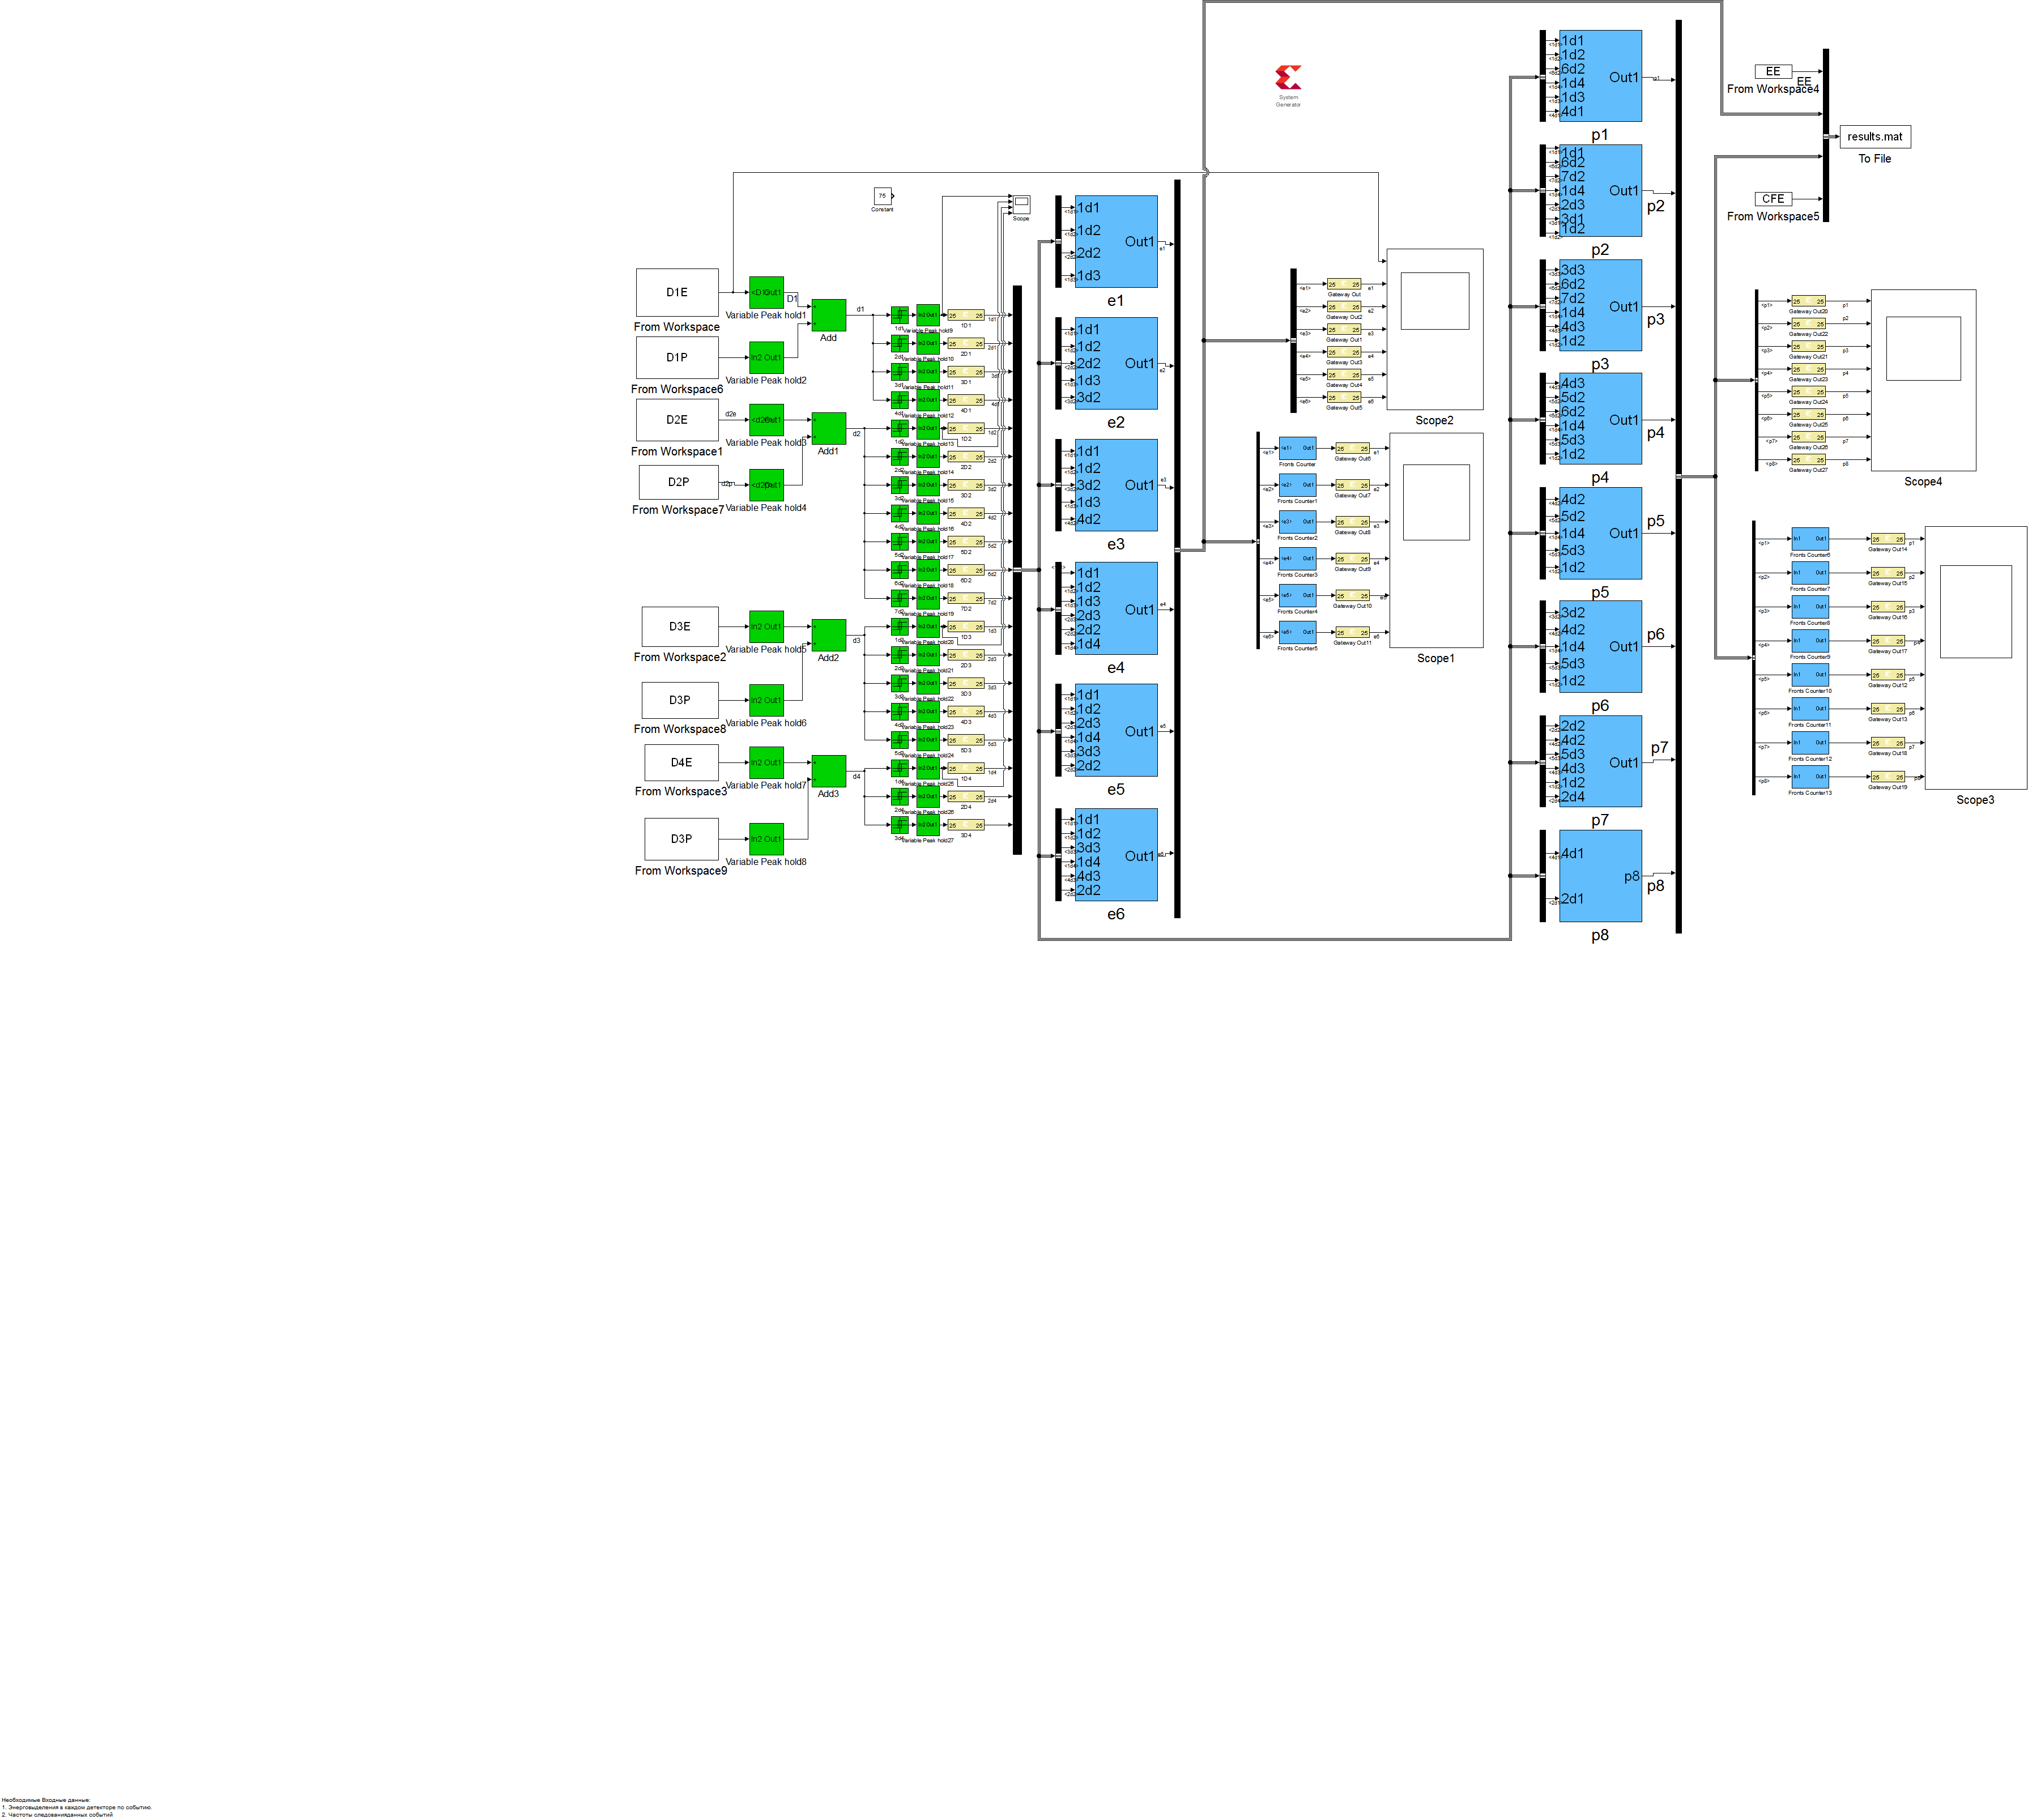
\includegraphics[width=0.7\linewidth]{images/simulink}
%	\caption{Общий вид модели прибора СПЭ в среде Simulink/Matlab. Логика определения типа и энергии частиц сгруппирована в подсистемы: е1-е6 структурные схемы выделения элекронов,  p1-p8 структурные схемы выделения протонов. D1…4E – промоделированные массивы энерговыделений в детекторах от электронов, D1…4P -  промоделированные массивы энерговыделений в детекторах от протонов. Блоки scope1-scope4 – виртуальные осциллографы в среде MATLAB, обеспечивающие наглядное отображение реакции исследуемого устройства на задаваемые внешние сигналы. Зеленым цветом показаны подсистемы имитации аналоговых сигналов, голубым цветом – подсистемы предназначенные для трансляции в аппаратный код ПЛИС, желтым цветом – выводы ПЛИС.}
%	\label{fig:simulink}
%\end{figure}

\chapter{Листинги программного кода комплекса ДЭПРОН} \label{AppendixB}


По причине проблем с поддержкой кириллицы (она встречается в комментариях и
печатаемых сообщениях), комментарии не отображены ~\ref{list:datecor}.
%\renewcommand\FBbskip{-20pt} % если хотим притянуть что-то к плавающему окружению из floatrow
Процедура \texttt{Detectors\_Handling} является основной процедурой цифровой обработки данных детекторов Дэпрон.
% далее метка для ссылки:
\label{list:Detectors_Handling}
\begin{lstlisting}[language={[ISO]C++}]
void Detectors_Handling(void)
{  
  int J, K;
  if (!Detectors_Flugs) {
    long interrupt_register = AT91C_BASE_PIOB->PIO_ISR;    
    return;
  }  
  Temporal_buff.FLUGS = Detectors_Flugs;
  if (Detectors_Flugs & Detec_Flug_ADC){
    dataADC = External_ADC_Read_Double();
    Temporal_buff.ADC_code = dataADC;
  } else dataADC = 0;

	
     if (Detectors_Flugs & Detec_Flug_compar){
     Prot_Comp_1++;  Prot_Comp_2++;  
        J= (((dataADC+3)>>3) & 0X00000FFF);
        Dose_Comp_1+=J;
        K= Digital_Compression(J);
        if (K<2) K=2; if(K>63) K=63;
        Spectra[2][K]++;
    
        J= (((dataADC+0x00030000)>>19) & 0X00000FFF);   //(short )
        Dose_Comp_2+=J;
        K= Digital_Compression(J);
        if (K<2) K=2; if(K>63) K=63;
        Spectra[3][K]++;

   } else {
	if ((Detectors_Flugs & Detec_Flug_P1)&&( dataADC & 0X00003FF0)){
        J= (((dataADC+3)>>3) & 0X00000FFF);
        Dose_1+=J;  Prot_1++;
        K= Digital_Compression(J);
        if (K<2) K=2; if(K>63) K=63;
        Spectra[0][K]++;
	}
	if ((Detectors_Flugs & Detec_Flug_P2)&&( dataADC & 0X3FF00000)){
        J= (((dataADC+0x00030000)>>19) & 0X00000FFF);
        Dose_2+=J;  Prot_2++;
        K= Digital_Compression(J);
        if (K<2) K=2; if(K>63) K=63;
        Spectra[1][K]++;
        }
  }
   if (Detectors_Flugs & Detec_Flug_N1){      
      Neutron_1 += Neut_1;
      Neut_1 = 0;
  } 
 
    if (Detectors_Flugs & Detec_Flug_N2){       
      Neutron_2 += Neut_2; 
      Neut_2 = 0;
  } 

//  if(Temporal_buff.interr_reg & Detector_Interrupt_t1) {
  if(Detectors_Flugs & Detec_Flug_T1_stop) {
    if(High_Ampl_Buffer.ind==0){
        High_Ampl_Buffer.day[0]= t_info.day;
        High_Ampl_Buffer.day[1]= t_info.Mounth;
    }    
    High_Ampl_Buffer.HA[High_Ampl_Buffer.ind].ADC_code = dataADC;
    High_Ampl_Buffer.HA[High_Ampl_Buffer.ind].ta[0] = tick_1;
    High_Ampl_Buffer.HA[High_Ampl_Buffer.ind].ta[1] = t_info.secunde;
    High_Ampl_Buffer.HA[High_Ampl_Buffer.ind].ta[2] = t_info.minute;
    High_Ampl_Buffer.HA[High_Ampl_Buffer.ind].ta[3] = t_info.hour;
    High_Ampl_Buffer.ind++;
    if(High_Ampl_Buffer.ind>62) Send_High_Ampl_Buffer();    
  }     
 //For Neutron burst 
   unsigned long N_T;
   unsigned short millisec_time = AT91C_BASE_TC2->TC_CV;
   millisec_time = millisec_time >>3;   //40 kHz / 8 = 5 kHz
    if ((Pronon_Fon < Proton_Level) && (N_ind > 0) && (Detectors_Flugs & Detec_Flug_Neutron)){      
      if (((millisec_time - Old_Tick_2)< D_tick_2) && (Old_Sec== t_info.day_second)){
        N_T= t_info.day_second <<15;
        N_T |= Old_Tick_2 & 0x00001fff;
        if (Detectors_Flugs & Detec_Flug_N1) N_T |= 0x00002000;
        if (Detectors_Flugs & Detec_Flug_N2) N_T |= 0x00004000;
        Neutron_Bunch.neutron_t[i_n_t++]=N_T;
        if(i_n_t>126) Send_Neutron_Bunch();
      }
    }
    Old_Sec = t_info.day_second;
    Old_Tick_2 = millisec_time;        
   
  
  Detectors_Flugs=0;

}	
\end{lstlisting}




\begin{ListingEnv}[H]
	% элементы, которые нежелательно разрывать обычно не ставят
	% посреди страницы: вместо H используется t (top, сверху страницы),
	% или b (bottom) или p (page, на отдельной странице)
	%    \captionsetup{format=tablenocaption}% должен стоять до самого caption
	%    \thisfloatsetup{\capposition=top}%
	\caption{Алгоритм коррекции даты в начале нового месяца на языке R}
	% далее метка для ссылки:
	\label{list:datecor}
	\begin{lstlisting}[language={Renhanced}]
	# date correction---------------------------------------------------------
	
	data.sec<-separate(data.sec, 'YYYY-MM-DD hh:mm:ss-1s',c("date", "time"),
	sep=' ')
	data.sec<-separate(data.sec, 'date',c("year", "month", "day"),
	sep='-', convert = TRUE)
	# изготовление даты из года и месяца, первого дня месяца и 12:00 по 
	умолчанию
	data.sec$dates <- ISOdate(data.sec$year, data.sec$month, 1)
	# получение правильного дня из дня который вышел за границы месяца
	data.sec$dates <- data.sec$dates + (as.integer(data.sec$day) - 1) * 60*60*24
	# установка 00:00  
	data.sec$dates <- data.sec$dates - 60*60*12 
	# установка вермени по часам прибора
	data.sec$dates <- data.sec$dates + parse_time(data.sec$time)
	
	\end{lstlisting}
\end{ListingEnv}

%\lstset{% general command to set parameter(s)
%	basicstyle=\footnotesize} % print whole listing small

\begin{ListingEnv}[H]	
	\caption{Алгоритм коррекции ухода 
		приборных часов на R}

	\label{list:timecor}
	\begin{lstlisting}[language={Renhanced}, ]
	\end{lstlisting}
\end{ListingEnv}

\begin{lstlisting}[language={Renhanced}, ]
# time correction------------------------------------------------------------

data.sec <- data.sec%>%
mutate(dates.UTC = data.sec$dates  - 60*60*3 )

data.sec <- data.sec[,(-17:-22)]

# константа постоянного ухода часов прибора
kt = (56.77315002) /86400

# вычитание постоянного ухода часов прибора
data.sec <- data.sec %>%
mutate(dates.correct.benghin =  dates.UTC - ceiling(
		kt* (dates.UTC - min(dates.UTC))
		))

# восстановление времени начала записи в файл
data.sec$timestamp.start <-gsub("depron-","0x",data.sec$filename)
data.sec$timestamp.start <-gsub(".dat","",data.sec$timestamp.start)
data.sec$timestamp.start <- as.POSIXct(as.integer(data.sec$timestamp.start), 
origin="1970-01-01", 'GMT' )

# восстановление времни последней записи в файл
data.sec$timestamp.end <- 
	as.POSIXct(strptime(data.sec$timestamp,format="%d.%m.%Y %H:%M"))

# получени разности между началом файла и горизонтальным приборным временем
data.sec$time.delta.file.start <- as.numeric(data.sec$dates.correct.benghin - 
data.sec$timestamp.start ,
units = "secs") 

data.sec <- data.sec %>%
	group_by(filename) %>%
	distinct(filename) %>%
	summarise(delta.minimum = min(time.delta.file.start)) %>%
	left_join(data.sec, ., by = 'filename')

# table(data.sec$delta.minimum)
data.sec$time.correct.zolotarev <- data.sec$dates.correct.benghin - 
data.sec$delta.minimum 

# отбор перескоков времени в приборе более 120 с - меньшие значения возможны 
при нормальной работе, 
# большие только при отключениях питания
data.sec <-mutate(data.sec, lag.delta = delta.minimum - lag(delta.minimum))
table(data.sec$lag.delta)
data.sec.switches <-filter(data.sec, abs(lag.delta) >120)

data.sec <-  data.sec %>%
	mutate(switches = cut(data.sec$dates.UTC, 
	breaks = c(min(data.sec$dates.UTC),
	data.sec.switches$dates.UTC,
	max(data.sec$dates.UTC) )))

# xy1 <- xyplot( delta.minimum + switches ~ timestamp.start , data = data.sec,
#                type = c("o","g"))
# plot(xy1)

# plot(table(data.sec$delta.minimum))
# table(data.sec$delta.minimum)
# median(data.sec$delta.minimum)
# mfv(data.sec$delta.minimum)

library('modeest')
if(nrow(data.sec.switches)>0){
	data.sec <-  data.sec %>%
		group_by(switches)  %>%
		mutate(mfv.delta =max(mfv(delta.minimum)))
}
if(nrow(data.sec.switches)== 0){
	data.sec <-  data.sec %>%
	mutate(mfv.delta =max(mfv(delta.minimum)))
}

data.sec <-  data.sec %>%
	mutate(dates.correct = dates.correct.benghin - mfv.delta)

# минус минута так как данные приходят по окончании минуты
data.sec$dates.correct <- as.POSIXct(data.sec$dates.correct, 'GMT') - 59

data.sec$dates.correct.copy <- as.POSIXct(data.sec$dates.correct, 'GMT')
# последняя проверка
# получениЕ разности между началом файла и правильным временем
data.sec$correct.time.delta.file.start <- as.numeric(data.sec$dates.correct - 
data.sec$timestamp.start, units = "secs")
\end{lstlisting}

%
%Листинг~\ref{list:external1} подгружается из внешнего файла. Приходится 
%загружать без окружения дополнительного. Иначе по страницам не переносится.
%
%\lstinputlisting[firstline=133,lastline=178,language={R},
%caption={Листинг из 
%	внешнего файла}]{./listings/save_depron_data.R}
%
%\lstinputlisting[firstline=179,lastline=318,language={Renhanced},inputencoding=cp1251,
%caption={Листинг из 
%внешнего файла},label={list:external1}]{./listings/save_depron_data.R}



\chapter{Листинги программного кода моделирования ДЭПРОН} \label{AppendixС}
\begin{lstlisting}[language=XML, firstline=1, lastline=89]
<?xml version="1.0" encoding="UTF-8"?>

<gdml xmlns:xsi="http://www.w3.org/2001/XMLSchema-instance" xsi:noNamespaceSchemaLocation="http://service-spi.web.cern.ch/service-spi/app/releases/GDML/schema/gdml.xsd">
<define>
<position name="central" x="0" y="0" z="0" unit="mm"/>
<rotation name="identity" x="0" y="0" z="0" unit="degree"/>
<variable name="DEGtoRAD" value="1.74532925199433E-02"/>
</define>
<materials>

<isotope name="he3_iso" Z="2" N="3">
<atom type="A" value="3.0160293"/>
</isotope> 


<element name="he3_ele" >
<fraction n="1" ref="he3_iso" />
</element>


<material formula="he" name="He3" >
<D value="0.00066975" />
<fraction n="1" ref="he3_ele" />
</material>


<material name="PCB" state="solid">
<D value="2.31"  unit="g/cm3"/>
<!--//pcbNchip Cu9Si5C460H506O138 epoxy + silicon + copper
//weight ratio 57.7:4:1
density = 2.31*g/cm3;
pcbNchip = new G4Material(name="Pcb&Chip", density, nElem=5);
pcbNchip->AddElement(elH, nAtoms=506);
pcbNchip->AddElement(elC, nAtoms=460);
pcbNchip->AddElement(elO, nAtoms=138);
pcbNchip->AddElement(elSi, nAtoms=5);
pcbNchip->AddElement(elCu, nAtoms=9);-->
<fraction n="0.056951255" ref="G4_H"/>
<!-- 1.00794*506=510.01764-->
<fraction n="0.616957286" ref="G4_C"/>
<!-- 12.011*460=5525.06-->
<fraction n="0.246547658" ref="G4_O"/>
<!-- 15.9994*138=2207.9172-->
<fraction n="0.015680874" ref="G4_Si"/>
<!-- 28.0855*5=140.4275-->
<fraction n="0.063862928" ref="G4_Cu"/>
<!-- 63.546*9=571.914-->
<!-- Total 8955.33634-->
</material>

<material name="D16" state="solid">
<D value="2.77"  unit="g/cm3"/>
<!--//aluminium alloy d16
Fe	Si	Mn		Cr	Ti	Al		Cu		Mg		Zn	Other				-
<0.5	<0.5	0.3 - 0.9	<0.1	<0.15	90.9 - 94.7	3.8 - 4.9	1.2 - 1.8	<0.25	all other 0.05; total 0.15	Ti+Zr < 0.2
G4Material::AddMaterial WARNING !! for D16 sum of fractional masses 0.0874738 is not 1 - results may be wrong
-->
<fraction n="0.0050"  ref="G4_Fe"/>
<fraction n="0.0050"  ref="G4_Si"/>
<fraction n="0.0090"  ref="G4_Mn"/>
<fraction n="0.9302"  ref="G4_Al"/>
<fraction n="0.0490"  ref="G4_Cu"/>
<fraction n="0.0018"  ref="G4_Mg"/>
</material>

</materials>
<solids>
<trd name="CoverVytochka_PartBody" x1="(1.5)*2" x2="(1.5)*2" y1="(30)*2" y2="(3)*2" z="(13.5)*2" lunit="mm"/>
<trd name="CoverVytochka2_PartBody" x1="(1.5)*2" x2="(1.5)*2" y1="(20)*2" y2="(0.001)*2" z="(10)*2" lunit="mm"/>
<box name="PCB1_PartBody" x="(0.75)*2" y="(25)*2" z="(17)*2" lunit="mm"/>
<box name="PCB2_PartBody" x="(20)*2" y="(40)*2" z="(0.75)*2" lunit="mm"/>
<tube name="PCB3hole_PartBody" rmin="0" rmax="5" z="(0.75)*2" startphi="0" deltaphi="360" lunit="mm" aunit="degree"/>
<box name="PCB3_PartBody" x="(0.75)*2" y="(25)*2" z="(17)*2" lunit="mm"/>
<tube name="si13tube_PartBody" rmin="15" rmax="16" z="(85)*2" startphi="0" deltaphi="360" lunit="mm" aunit="degree"/>
<tube name="si13n_PartBody" rmin="0" rmax="15" z="(95)*2" startphi="0" deltaphi="360" lunit="mm" aunit="degree"/>
<box name="Detector_PartBody" x="(5)*2" y="(5)*2" z="(0.15)*2" lunit="mm"/>
<box name="Detector_PartBody" x="(5)*2" y="(5)*2" z="(0.15)*2" lunit="mm"/>
<box name="G4Space_PartBody" x="(100)*2" y="(16)*2" z="(16)*2" lunit="mm"/>
<box name="Shield_PartBody" x="(110)*2" y="(24.5)*2" z="(24.5)*2" lunit="mm"/>
<box name="CoverFront2_PartBody" x="(2.5)*2" y="(75)*2" z="(35)*2" lunit="mm"/>
<box name="CoverSide_PartBody" x="(125)*2" y="(2.5)*2" z="(35)*2" lunit="mm"/>
<box name="CoverTop_PartBody" x="(125)*2" y="(80)*2" z="(2.5)*2" lunit="mm"/>
<box name="CoverBottom_PartBody" x="(125)*2" y="(80)*2" z="(2.5)*2" lunit="mm"/>
<box name="casset_cover_front_PartBody" x="(0.05)*2" y="(25)*2" z="(17)*2" lunit="mm"/>
<box name="casset_cover_top_PartBody" x="(50)*2" y="(26)*2" z="(0.15)*2" lunit="mm"/>
<box name="casset_cover_side_PartBody" x="(50)*2" y="(0.25)*2" z="(17)*2" lunit="mm"/>
<box name="cassete_cover_top_vert_PartBody" x="(0.15)*2" y="(26)*2" z="(33)*2" lunit="mm"/>
<box name="casset_cover_side_vert_PartBody" x="(17)*2" y="(0.25)*2" z="(33)*2" lunit="mm"/>
<box name="G4Cover_PartBody" x="(125)*2" y="(80)*2" z="(41)*2" lunit="mm"/>
<box name="G4World_PartBody" x="(1000)*2" y="(1000)*2" z="(1000)*2" lunit="mm"/>
</solids>
<structure>
<volume name="CoverVytochka">
<materialref ref="G4_AIR"/>
<solidref ref="CoverVytochka_PartBody"/>
</volume>
<volume name="CoverVytochka2">
<materialref ref="G4_AIR"/>
<solidref ref="CoverVytochka2_PartBody"/>
</volume>
<volume name="PCB1">
<materialref ref="PCB"/>
<solidref ref="PCB1_PartBody"/>
</volume>
<volume name="PCB2">
<materialref ref="PCB"/>
<solidref ref="PCB2_PartBody"/>
</volume>
<volume name="PCB3hole">
<materialref ref="G4_AIR"/>
<solidref ref="PCB3hole_PartBody"/>
</volume>
<volume name="PCB3">
<materialref ref="PCB"/>
<solidref ref="PCB3_PartBody"/>
<physvol>
<volumeref ref="PCB3hole"/>
<position name="PCB3_pos_PCB3hole_1" x="0" y="10" z="0" unit="mm"/>
<rotation name="PCB3_rot_PCB3hole_1" x="0" y="-90" z="0" unit="degree"/>
</physvol>
</volume>
<volume name="si13tube">
<materialref ref="G4_Fe"/>
<solidref ref="si13tube_PartBody"/>
</volume>
<volume name="si13n1">
<materialref ref="He3"/>
<solidref ref="si13n_PartBody"/>
</volume>

<volume name="si13n2">

<materialref ref="He3"/>

<solidref ref="si13n_PartBody"/>

</volume>
<volume name="Detector1">
<materialref ref="G4_Si"/>
<solidref ref="Detector_PartBody"/>
</volume>
<volume name="Detector2">
<materialref ref="G4_Si"/>
<solidref ref="Detector_PartBody"/>
</volume>
<volume name="G4Space">
<materialref ref="G4_AIR"/>
<solidref ref="G4Space_PartBody"/>
<physvol>
<volumeref ref="si13n1"/>
<position name="G4Space_pos_si13n_1" x="0" y="0" z="0" unit="mm"/>
<rotation name="G4Space_rot_si13n_1" x="0" y="-90" z="0" unit="degree"/>
</physvol>
<physvol>
<volumeref ref="si13tube"/>
<position name="G4Space_pos_si13tube_1" x="0" y="0" z="0" unit="mm"/>
<rotation name="G4Space_rot_si13tube_1" x="0" y="-90" z="0" unit="degree"/>
</physvol>
</volume>
<volume name="Shield">
<materialref ref="G4_PLEXIGLASS"/>
<solidref ref="Shield_PartBody"/>
<physvol>
<volumeref ref="G4Space"/>
<position name="Shield_pos_G4Space_1" x="0" y="0" z="0" unit="mm"/>
<rotation name="Shield_rot_G4Space_1" x="0" y="0" z="0" unit="degree"/>
</physvol>
</volume>
<volume name="CoverFront2">
<materialref ref="D16"/>
<solidref ref="CoverFront2_PartBody"/>
<physvol>
<volumeref ref="CoverVytochka2"/>
<position name="CoverFront2__pos__CoverVytochka2_0" x="-1" y="-60.57" z=" 24" unit="mm"/>
<rotation name="CoverFront2__rot__CoverVytochka2_0" x="-45" y=" 0" z=" 0" unit="deg"/>
</physvol>
<physvol>
<volumeref ref="CoverVytochka2"/>
<position name="CoverFront2__pos__CoverVytochka2_1" x="-1" y="-24.57" z=" 24" unit="mm"/>
<rotation name="CoverFront2__rot__CoverVytochka2_1" x="-45" y=" 0" z=" 0" unit="deg"/>
</physvol>
<physvol>
<volumeref ref="CoverVytochka2"/>
<position name="CoverFront2__pos__CoverVytochka2_2" x="-1" y=" 11.43" z=" 24" unit="mm"/>
<rotation name="CoverFront2__rot__CoverVytochka2_2" x="-45" y=" 0" z=" 0" unit="deg"/>
</physvol>
<physvol>
<volumeref ref="CoverVytochka2"/>
<position name="CoverFront2__pos__CoverVytochka2_3" x="-1" y=" 47.43" z=" 24" unit="mm"/>
<rotation name="CoverFront2__rot__CoverVytochka2_3" x="-45" y=" 0" z=" 0" unit="deg"/>
</physvol>
<physvol>
<volumeref ref="CoverVytochka2"/>
<position name="CoverFront2__pos__CoverVytochka2_0" x="-1" y="-46.428" z=" 8.858" unit="mm"/>
<rotation name="CoverFront2__rot__CoverVytochka2_0" x=" 135" y=" 0" z=" 0" unit="deg"/>
</physvol>
<physvol>
<volumeref ref="CoverVytochka2"/>
<position name="CoverFront2__pos__CoverVytochka2_1" x="-1" y="-10.428" z=" 8.858" unit="mm"/>
<rotation name="CoverFront2__rot__CoverVytochka2_1" x=" 135" y=" 0" z=" 0" unit="deg"/>
</physvol>
<physvol>
<volumeref ref="CoverVytochka2"/>
<position name="CoverFront2__pos__CoverVytochka2_2" x="-1" y=" 25.572" z=" 8.858" unit="mm"/>
<rotation name="CoverFront2__rot__CoverVytochka2_2" x=" 135" y=" 0" z=" 0" unit="deg"/>
</physvol>
<physvol>
<volumeref ref="CoverVytochka2"/>
<position name="CoverFront2__pos__CoverVytochka2_3" x="-1" y=" 61.572" z=" 8.858" unit="mm"/>
<rotation name="CoverFront2__rot__CoverVytochka2_3" x=" 135" y=" 0" z=" 0" unit="deg"/>
</physvol>
<physvol>
<volumeref ref="CoverVytochka2"/>
<position name="CoverFront2__pos__CoverVytochka2_0" x="-1" y="-60.571" z="-9.285" unit="mm"/>
<rotation name="CoverFront2__rot__CoverVytochka2_0" x="-45" y=" 0" z=" 0" unit="deg"/>
</physvol>
<physvol>
<volumeref ref="CoverVytochka2"/>
<position name="CoverFront2__pos__CoverVytochka2_1" x="-1" y="-24.571" z="-9.285" unit="mm"/>
<rotation name="CoverFront2__rot__CoverVytochka2_1" x="-45" y=" 0" z=" 0" unit="deg"/>
</physvol>
<physvol>
<volumeref ref="CoverVytochka2"/>
<position name="CoverFront2__pos__CoverVytochka2_2" x="-1" y=" 11.429" z="-9.285" unit="mm"/>
<rotation name="CoverFront2__rot__CoverVytochka2_2" x="-45" y=" 0" z=" 0" unit="deg"/>
</physvol>
<physvol>
<volumeref ref="CoverVytochka2"/>
<position name="CoverFront2__pos__CoverVytochka2_3" x="-1" y=" 47.429" z="-9.285" unit="mm"/>
<rotation name="CoverFront2__rot__CoverVytochka2_3" x="-45" y=" 0" z=" 0" unit="deg"/>
</physvol>
<physvol>
<volumeref ref="CoverVytochka2"/>
<position name="CoverFront2__pos__CoverVytochka2_0" x="-1" y="-46.429" z="-24.427" unit="mm"/>
<rotation name="CoverFront2__rot__CoverVytochka2_0" x=" 135" y=" 0" z=" 0" unit="deg"/>
</physvol>
<physvol>
<volumeref ref="CoverVytochka2"/>
<position name="CoverFront2__pos__CoverVytochka2_1" x="-1" y="-10.429" z="-24.427" unit="mm"/>
<rotation name="CoverFront2__rot__CoverVytochka2_1" x=" 135" y=" 0" z=" 0" unit="deg"/>
</physvol>
<physvol>
<volumeref ref="CoverVytochka2"/>
<position name="CoverFront2__pos__CoverVytochka2_2" x="-1" y=" 25.571" z="-24.427" unit="mm"/>
<rotation name="CoverFront2__rot__CoverVytochka2_2" x=" 135" y=" 0" z=" 0" unit="deg"/>
</physvol>
<physvol>
<volumeref ref="CoverVytochka2"/>
<position name="CoverFront2__pos__CoverVytochka2_3" x="-1" y=" 61.571" z="-24.427" unit="mm"/>
<rotation name="CoverFront2__rot__CoverVytochka2_3" x=" 135" y=" 0" z=" 0" unit="deg"/>
</physvol>
</volume>
<volume name="CoverSide">
<materialref ref="D16"/>
<solidref ref="CoverSide_PartBody"/>
<physvol>
<volumeref ref="CoverVytochka2"/>
<position name="CoverSide__pos__CoverVytochka2_0" x="-115.93" y="-1" z=" 25.928" unit="mm"/>
<rotation name="CoverSide__rot__CoverVytochka2_0" x=" 0" y=" 45" z="-90" unit="deg"/>
</physvol>
<physvol>
<volumeref ref="CoverVytochka2"/>
<position name="CoverSide__pos__CoverVytochka2_1" x="-79.93" y="-1" z=" 25.928" unit="mm"/>
<rotation name="CoverSide__rot__CoverVytochka2_1" x=" 0" y=" 45" z="-90" unit="deg"/>
</physvol>
<physvol>
<volumeref ref="CoverVytochka2"/>
<position name="CoverSide__pos__CoverVytochka2_2" x="-43.93" y="-1" z=" 25.928" unit="mm"/>
<rotation name="CoverSide__rot__CoverVytochka2_2" x=" 0" y=" 45" z="-90" unit="deg"/>
</physvol>
<physvol>
<volumeref ref="CoverVytochka2"/>
<position name="CoverSide__pos__CoverVytochka2_3" x="-7.93000000000001" y="-1" z=" 25.928" unit="mm"/>
<rotation name="CoverSide__rot__CoverVytochka2_3" x=" 0" y=" 45" z="-90" unit="deg"/>
</physvol>
<physvol>
<volumeref ref="CoverVytochka2"/>
<position name="CoverSide__pos__CoverVytochka2_4" x=" 28.07" y="-1" z=" 25.928" unit="mm"/>
<rotation name="CoverSide__rot__CoverVytochka2_4" x=" 0" y=" 45" z="-90" unit="deg"/>
</physvol>
<physvol>
<volumeref ref="CoverVytochka2"/>
<position name="CoverSide__pos__CoverVytochka2_5" x=" 64.07" y="-1" z=" 25.928" unit="mm"/>
<rotation name="CoverSide__rot__CoverVytochka2_5" x=" 0" y=" 45" z="-90" unit="deg"/>
</physvol>
<physvol>
<volumeref ref="CoverVytochka2"/>
<position name="CoverSide__pos__CoverVytochka2_6" x=" 100.07" y="-1" z=" 25.928" unit="mm"/>
<rotation name="CoverSide__rot__CoverVytochka2_6" x=" 0" y=" 45" z="-90" unit="deg"/>
</physvol>
<physvol>
<volumeref ref="CoverVytochka2"/>
<position name="CoverSide__pos__CoverVytochka2_0" x="-101.788" y="-1" z=" 10.786" unit="mm"/>
<rotation name="CoverSide__rot__CoverVytochka2_0" x=" 0" y="-135" z="-90" unit="deg"/>
</physvol>
<physvol>
<volumeref ref="CoverVytochka2"/>
<position name="CoverSide__pos__CoverVytochka2_1" x="-65.788" y="-1" z=" 10.786" unit="mm"/>
<rotation name="CoverSide__rot__CoverVytochka2_1" x=" 0" y="-135" z="-90" unit="deg"/>
</physvol>
<physvol>
<volumeref ref="CoverVytochka2"/>
<position name="CoverSide__pos__CoverVytochka2_2" x="-29.788" y="-1" z=" 10.786" unit="mm"/>
<rotation name="CoverSide__rot__CoverVytochka2_2" x=" 0" y="-135" z="-90" unit="deg"/>
</physvol>
<physvol>
<volumeref ref="CoverVytochka2"/>
<position name="CoverSide__pos__CoverVytochka2_3" x=" 6.212" y="-1" z=" 10.786" unit="mm"/>
<rotation name="CoverSide__rot__CoverVytochka2_3" x=" 0" y="-135" z="-90" unit="deg"/>
</physvol>
<physvol>
<volumeref ref="CoverVytochka2"/>
<position name="CoverSide__pos__CoverVytochka2_4" x=" 42.212" y="-1" z=" 10.786" unit="mm"/>
<rotation name="CoverSide__rot__CoverVytochka2_4" x=" 0" y="-135" z="-90" unit="deg"/>
</physvol>
<physvol>
<volumeref ref="CoverVytochka2"/>
<position name="CoverSide__pos__CoverVytochka2_5" x=" 78.212" y="-1" z=" 10.786" unit="mm"/>
<rotation name="CoverSide__rot__CoverVytochka2_5" x=" 0" y="-135" z="-90" unit="deg"/>
</physvol>
<physvol>
<volumeref ref="CoverVytochka2"/>
<position name="CoverSide__pos__CoverVytochka2_6" x=" 114.212" y="-1" z=" 10.786" unit="mm"/>
<rotation name="CoverSide__rot__CoverVytochka2_6" x=" 0" y="-135" z="-90" unit="deg"/>
</physvol>
<physvol>
<volumeref ref="CoverVytochka2"/>
<position name="CoverSide__pos__CoverVytochka2_0" x="-115.931" y="-1" z="-5.357" unit="mm"/>
<rotation name="CoverSide__rot__CoverVytochka2_0" x=" 0" y=" 45" z="-90" unit="deg"/>
</physvol>
<physvol>
<volumeref ref="CoverVytochka2"/>
<position name="CoverSide__pos__CoverVytochka2_1" x="-79.931" y="-1" z="-5.357" unit="mm"/>
<rotation name="CoverSide__rot__CoverVytochka2_1" x=" 0" y=" 45" z="-90" unit="deg"/>
</physvol>
<physvol>
<volumeref ref="CoverVytochka2"/>
<position name="CoverSide__pos__CoverVytochka2_2" x="-43.931" y="-1" z="-5.357" unit="mm"/>
<rotation name="CoverSide__rot__CoverVytochka2_2" x=" 0" y=" 45" z="-90" unit="deg"/>
</physvol>
<physvol>
<volumeref ref="CoverVytochka2"/>
<position name="CoverSide__pos__CoverVytochka2_3" x="-7.931" y="-1" z="-5.357" unit="mm"/>
<rotation name="CoverSide__rot__CoverVytochka2_3" x=" 0" y=" 45" z="-90" unit="deg"/>
</physvol>
<physvol>
<volumeref ref="CoverVytochka2"/>
<position name="CoverSide__pos__CoverVytochka2_4" x=" 28.069" y="-1" z="-5.357" unit="mm"/>
<rotation name="CoverSide__rot__CoverVytochka2_4" x=" 0" y=" 45" z="-90" unit="deg"/>
</physvol>
<physvol>
<volumeref ref="CoverVytochka2"/>
<position name="CoverSide__pos__CoverVytochka2_5" x=" 64.069" y="-1" z="-5.357" unit="mm"/>
<rotation name="CoverSide__rot__CoverVytochka2_5" x=" 0" y=" 45" z="-90" unit="deg"/>
</physvol>
<physvol>
<volumeref ref="CoverVytochka2"/>
<position name="CoverSide__pos__CoverVytochka2_6" x=" 100.069" y="-1" z="-5.357" unit="mm"/>
<rotation name="CoverSide__rot__CoverVytochka2_6" x=" 0" y=" 45" z="-90" unit="deg"/>
</physvol>
<physvol>
<volumeref ref="CoverVytochka2"/>
<position name="CoverSide__pos__CoverVytochka2_0" x="-101.789" y="-1" z="-20.499" unit="mm"/>
<rotation name="CoverSide__rot__CoverVytochka2_0" x=" 0" y="-135" z="-90" unit="deg"/>
</physvol>
<physvol>
<volumeref ref="CoverVytochka2"/>
<position name="CoverSide__pos__CoverVytochka2_1" x="-65.789" y="-1" z="-20.499" unit="mm"/>
<rotation name="CoverSide__rot__CoverVytochka2_1" x=" 0" y="-135" z="-90" unit="deg"/>
</physvol>
<physvol>
<volumeref ref="CoverVytochka2"/>
<position name="CoverSide__pos__CoverVytochka2_2" x="-29.789" y="-1" z="-20.499" unit="mm"/>
<rotation name="CoverSide__rot__CoverVytochka2_2" x=" 0" y="-135" z="-90" unit="deg"/>
</physvol>
<physvol>
<volumeref ref="CoverVytochka2"/>
<position name="CoverSide__pos__CoverVytochka2_3" x=" 6.211" y="-1" z="-20.499" unit="mm"/>
<rotation name="CoverSide__rot__CoverVytochka2_3" x=" 0" y="-135" z="-90" unit="deg"/>
</physvol>
<physvol>
<volumeref ref="CoverVytochka2"/>
<position name="CoverSide__pos__CoverVytochka2_4" x=" 42.211" y="-1" z="-20.499" unit="mm"/>
<rotation name="CoverSide__rot__CoverVytochka2_4" x=" 0" y="-135" z="-90" unit="deg"/>
</physvol>
<physvol>
<volumeref ref="CoverVytochka2"/>
<position name="CoverSide__pos__CoverVytochka2_5" x=" 78.211" y="-1" z="-20.499" unit="mm"/>
<rotation name="CoverSide__rot__CoverVytochka2_5" x=" 0" y="-135" z="-90" unit="deg"/>
</physvol>
<physvol>
<volumeref ref="CoverVytochka2"/>
<position name="CoverSide__pos__CoverVytochka2_6" x=" 114.211" y="-1" z="-20.499" unit="mm"/>
<rotation name="CoverSide__rot__CoverVytochka2_6" x=" 0" y="-135" z="-90" unit="deg"/>
</physvol>
</volume>
<volume name="CoverTop">
<materialref ref="D16"/>
<solidref ref="CoverTop_PartBody"/>
<physvol>
<volumeref ref="CoverVytochka"/>
<position name="CoverTop__pos__CoverVytochka_0" x="-93" y=" 24.5" z=" 1" unit="mm"/>
<rotation name="CoverTop__rot__CoverVytochka_0" x="-90" y=" 0" z="-90" unit="deg"/>
</physvol>
<physvol>
<volumeref ref="CoverVytochka"/>
<position name="CoverTop__pos__CoverVytochka_1" x="-31" y=" 24.5" z=" 1" unit="mm"/>
<rotation name="CoverTop__rot__CoverVytochka_1" x="-90" y=" 0" z="-90" unit="deg"/>
</physvol>
<physvol>
<volumeref ref="CoverVytochka"/>
<position name="CoverTop__pos__CoverVytochka_2" x=" 31" y=" 24.5" z=" 1" unit="mm"/>
<rotation name="CoverTop__rot__CoverVytochka_2" x="-90" y=" 0" z="-90" unit="deg"/>
</physvol>
<physvol>
<volumeref ref="CoverVytochka"/>
<position name="CoverTop__pos__CoverVytochka_3" x=" 93" y=" 24.5" z=" 1" unit="mm"/>
<rotation name="CoverTop__rot__CoverVytochka_3" x="-90" y=" 0" z="-90" unit="deg"/>
</physvol>
<physvol>
<volumeref ref="CoverVytochka"/>
<position name="CoverTop__pos__CoverVytochka_0" x="-93" y=" 56.5" z=" 1" unit="mm"/>
<rotation name="CoverTop__rot__CoverVytochka_0" x=" 90" y=" 0" z="-90" unit="deg"/>
</physvol>
<physvol>
<volumeref ref="CoverVytochka"/>
<position name="CoverTop__pos__CoverVytochka_1" x="-31" y=" 56.5" z=" 1" unit="mm"/>
<rotation name="CoverTop__rot__CoverVytochka_1" x=" 90" y=" 0" z="-90" unit="deg"/>
</physvol>
<physvol>
<volumeref ref="CoverVytochka"/>
<position name="CoverTop__pos__CoverVytochka_2" x=" 31" y=" 56.5" z=" 1" unit="mm"/>
<rotation name="CoverTop__rot__CoverVytochka_2" x=" 90" y=" 0" z="-90" unit="deg"/>
</physvol>
<physvol>
<volumeref ref="CoverVytochka"/>
<position name="CoverTop__pos__CoverVytochka_3" x=" 93" y=" 56.5" z=" 1" unit="mm"/>
<rotation name="CoverTop__rot__CoverVytochka_3" x=" 90" y=" 0" z="-90" unit="deg"/>
</physvol>
<physvol>
<volumeref ref="CoverVytochka"/>
<position name="CoverTop__pos__CoverVytochka_0" x="-93" y="-56.5" z=" 1" unit="mm"/>
<rotation name="CoverTop__rot__CoverVytochka_0" x="-90" y=" 0" z="-90" unit="deg"/>
</physvol>
<physvol>
<volumeref ref="CoverVytochka"/>
<position name="CoverTop__pos__CoverVytochka_1" x="-31" y="-56.5" z=" 1" unit="mm"/>
<rotation name="CoverTop__rot__CoverVytochka_1" x="-90" y=" 0" z="-90" unit="deg"/>
</physvol>
<physvol>
<volumeref ref="CoverVytochka"/>
<position name="CoverTop__pos__CoverVytochka_2" x=" 31" y="-56.5" z=" 1" unit="mm"/>
<rotation name="CoverTop__rot__CoverVytochka_2" x="-90" y=" 0" z="-90" unit="deg"/>
</physvol>
<physvol>
<volumeref ref="CoverVytochka"/>
<position name="CoverTop__pos__CoverVytochka_3" x=" 93" y="-56.5" z=" 1" unit="mm"/>
<rotation name="CoverTop__rot__CoverVytochka_3" x="-90" y=" 0" z="-90" unit="deg"/>
</physvol>
<physvol>
<volumeref ref="CoverVytochka"/>
<position name="CoverTop__pos__CoverVytochka_0" x="-93" y="-24.5" z=" 1" unit="mm"/>
<rotation name="CoverTop__rot__CoverVytochka_0" x=" 90" y=" 0" z="-90" unit="deg"/>
</physvol>
<physvol>
<volumeref ref="CoverVytochka"/>
<position name="CoverTop__pos__CoverVytochka_1" x="-31" y="-24.5" z=" 1" unit="mm"/>
<rotation name="CoverTop__rot__CoverVytochka_1" x=" 90" y=" 0" z="-90" unit="deg"/>
</physvol>
<physvol>
<volumeref ref="CoverVytochka"/>
<position name="CoverTop__pos__CoverVytochka_2" x=" 31" y="-24.5" z=" 1" unit="mm"/>
<rotation name="CoverTop__rot__CoverVytochka_2" x=" 90" y=" 0" z="-90" unit="deg"/>
</physvol>
<physvol>
<volumeref ref="CoverVytochka"/>
<position name="CoverTop__pos__CoverVytochka_3" x=" 93" y="-24.5" z=" 1" unit="mm"/>
<rotation name="CoverTop__rot__CoverVytochka_3" x=" 90" y=" 0" z="-90" unit="deg"/>
</physvol>
<physvol>
<volumeref ref="CoverVytochka"/>
<position name="CoverTop__pos__CoverVytochka_0" x="-62" y=" 62" z=" 1" unit="mm"/>
<rotation name="CoverTop__rot__CoverVytochka_0" x="-90" y=" 0" z="-90" unit="deg"/>
</physvol>
<physvol>
<volumeref ref="CoverVytochka"/>
<position name="CoverTop__pos__CoverVytochka_1" x=" 0" y=" 62" z=" 1" unit="mm"/>
<rotation name="CoverTop__rot__CoverVytochka_1" x="-90" y=" 0" z="-90" unit="deg"/>
</physvol>
<physvol>
<volumeref ref="CoverVytochka"/>
<position name="CoverTop__pos__CoverVytochka_2" x=" 62" y=" 62" z=" 1" unit="mm"/>
<rotation name="CoverTop__rot__CoverVytochka_2" x="-90" y=" 0" z="-90" unit="deg"/>
</physvol>
<physvol>
<volumeref ref="CoverVytochka"/>
<position name="CoverTop__pos__CoverVytochka_0" x="-62" y="-62" z=" 1" unit="mm"/>
<rotation name="CoverTop__rot__CoverVytochka_0" x=" 90" y=" 0" z="-90" unit="deg"/>
</physvol>
<physvol>
<volumeref ref="CoverVytochka"/>
<position name="CoverTop__pos__CoverVytochka_1" x=" 0" y="-62" z=" 1" unit="mm"/>
<rotation name="CoverTop__rot__CoverVytochka_1" x=" 90" y=" 0" z="-90" unit="deg"/>
</physvol>
<physvol>
<volumeref ref="CoverVytochka"/>
<position name="CoverTop__pos__CoverVytochka_2" x=" 62" y="-62" z=" 1" unit="mm"/>
<rotation name="CoverTop__rot__CoverVytochka_2" x=" 90" y=" 0" z="-90" unit="deg"/>
</physvol>
<physvol>
<volumeref ref="CoverVytochka"/>
<position name="CoverTop__pos__CoverVytochka_0" x="-62" y=" 19" z=" 1" unit="mm"/>
<rotation name="CoverTop__rot__CoverVytochka_0" x=" 90" y=" 0" z="-90" unit="deg"/>
</physvol>
<physvol>
<volumeref ref="CoverVytochka"/>
<position name="CoverTop__pos__CoverVytochka_1" x=" 0" y=" 19" z=" 1" unit="mm"/>
<rotation name="CoverTop__rot__CoverVytochka_1" x=" 90" y=" 0" z="-90" unit="deg"/>
</physvol>
<physvol>
<volumeref ref="CoverVytochka"/>
<position name="CoverTop__pos__CoverVytochka_2" x=" 62" y=" 19" z=" 1" unit="mm"/>
<rotation name="CoverTop__rot__CoverVytochka_2" x=" 90" y=" 0" z="-90" unit="deg"/>
</physvol>
<physvol>
<volumeref ref="CoverVytochka"/>
<position name="CoverTop__pos__CoverVytochka_0" x="-62" y="-19" z=" 1" unit="mm"/>
<rotation name="CoverTop__rot__CoverVytochka_0" x="-90" y=" 0" z="-90" unit="deg"/>
</physvol>
<physvol>
<volumeref ref="CoverVytochka"/>
<position name="CoverTop__pos__CoverVytochka_1" x=" 0" y="-19" z=" 1" unit="mm"/>
<rotation name="CoverTop__rot__CoverVytochka_1" x="-90" y=" 0" z="-90" unit="deg"/>
</physvol>
<physvol>
<volumeref ref="CoverVytochka"/>
<position name="CoverTop__pos__CoverVytochka_2" x=" 62" y="-19" z=" 1" unit="mm"/>
<rotation name="CoverTop__rot__CoverVytochka_2" x="-90" y=" 0" z="-90" unit="deg"/>
</physvol>
</volume>
<volume name="CoverBottom">
<materialref ref="D16"/>
<solidref ref="CoverBottom_PartBody"/>
<physvol>
<volumeref ref="CoverVytochka"/>
<position name="CoverBottom__pos__CoverVytochka_0" x="-93" y=" 24.5" z=" 1" unit="mm"/>
<rotation name="CoverBottom__rot__CoverVytochka_0" x="-90" y=" 0" z="-90" unit="deg"/>
</physvol>
<physvol>
<volumeref ref="CoverVytochka"/>
<position name="CoverBottom__pos__CoverVytochka_1" x="-31" y=" 24.5" z=" 1" unit="mm"/>
<rotation name="CoverBottom__rot__CoverVytochka_1" x="-90" y=" 0" z="-90" unit="deg"/>
</physvol>
<physvol>
<volumeref ref="CoverVytochka"/>
<position name="CoverBottom__pos__CoverVytochka_2" x=" 31" y=" 24.5" z=" 1" unit="mm"/>
<rotation name="CoverBottom__rot__CoverVytochka_2" x="-90" y=" 0" z="-90" unit="deg"/>
</physvol>
<physvol>
<volumeref ref="CoverVytochka"/>
<position name="CoverBottom__pos__CoverVytochka_3" x=" 93" y=" 24.5" z=" 1" unit="mm"/>
<rotation name="CoverBottom__rot__CoverVytochka_3" x="-90" y=" 0" z="-90" unit="deg"/>
</physvol>
<physvol>
<volumeref ref="CoverVytochka"/>
<position name="CoverBottom__pos__CoverVytochka_0" x="-93" y=" 56.5" z=" 1" unit="mm"/>
<rotation name="CoverBottom__rot__CoverVytochka_0" x="-90" y="-180" z="-90" unit="deg"/>
</physvol>
<physvol>
<volumeref ref="CoverVytochka"/>
<position name="CoverBottom__pos__CoverVytochka_1" x="-31" y=" 56.5" z=" 1" unit="mm"/>
<rotation name="CoverBottom__rot__CoverVytochka_1" x="-90" y="-180" z="-90" unit="deg"/>
</physvol>
<physvol>
<volumeref ref="CoverVytochka"/>
<position name="CoverBottom__pos__CoverVytochka_2" x=" 31" y=" 56.5" z=" 1" unit="mm"/>
<rotation name="CoverBottom__rot__CoverVytochka_2" x="-90" y="-180" z="-90" unit="deg"/>
</physvol>
<physvol>
<volumeref ref="CoverVytochka"/>
<position name="CoverBottom__pos__CoverVytochka_3" x=" 93" y=" 56.5" z=" 1" unit="mm"/>
<rotation name="CoverBottom__rot__CoverVytochka_3" x="-90" y="-180" z="-90" unit="deg"/>
</physvol>
<physvol>
<volumeref ref="CoverVytochka"/>
<position name="CoverBottom__pos__CoverVytochka_0" x="-93" y="-56.5" z=" 1" unit="mm"/>
<rotation name="CoverBottom__rot__CoverVytochka_0" x="-90" y=" 0" z="-90" unit="deg"/>
</physvol>
<physvol>
<volumeref ref="CoverVytochka"/>
<position name="CoverBottom__pos__CoverVytochka_1" x="-31" y="-56.5" z=" 1" unit="mm"/>
<rotation name="CoverBottom__rot__CoverVytochka_1" x="-90" y=" 0" z="-90" unit="deg"/>
</physvol>
<physvol>
<volumeref ref="CoverVytochka"/>
<position name="CoverBottom__pos__CoverVytochka_2" x=" 31" y="-56.5" z=" 1" unit="mm"/>
<rotation name="CoverBottom__rot__CoverVytochka_2" x="-90" y=" 0" z="-90" unit="deg"/>
</physvol>
<physvol>
<volumeref ref="CoverVytochka"/>
<position name="CoverBottom__pos__CoverVytochka_3" x=" 93" y="-56.5" z=" 1" unit="mm"/>
<rotation name="CoverBottom__rot__CoverVytochka_3" x="-90" y=" 0" z="-90" unit="deg"/>
</physvol>
<physvol>
<volumeref ref="CoverVytochka"/>
<position name="CoverBottom__pos__CoverVytochka_0" x="-93" y="-24.5" z=" 1" unit="mm"/>
<rotation name="CoverBottom__rot__CoverVytochka_0" x="-90" y="-180" z="-90" unit="deg"/>
</physvol>
<physvol>
<volumeref ref="CoverVytochka"/>
<position name="CoverBottom__pos__CoverVytochka_1" x="-31" y="-24.5" z=" 1" unit="mm"/>
<rotation name="CoverBottom__rot__CoverVytochka_1" x="-90" y="-180" z="-90" unit="deg"/>
</physvol>
<physvol>
<volumeref ref="CoverVytochka"/>
<position name="CoverBottom__pos__CoverVytochka_2" x=" 31" y="-24.5" z=" 1" unit="mm"/>
<rotation name="CoverBottom__rot__CoverVytochka_2" x="-90" y="-180" z="-90" unit="deg"/>
</physvol>
<physvol>
<volumeref ref="CoverVytochka"/>
<position name="CoverBottom__pos__CoverVytochka_3" x=" 93" y="-24.5" z=" 1" unit="mm"/>
<rotation name="CoverBottom__rot__CoverVytochka_3" x="-90" y="-180" z="-90" unit="deg"/>
</physvol>
<physvol>
<volumeref ref="CoverVytochka"/>
<position name="CoverBottom__pos__CoverVytochka_0" x="-62" y=" 62" z=" 1" unit="mm"/>
<rotation name="CoverBottom__rot__CoverVytochka_0" x="-90" y=" 0" z="-90" unit="deg"/>
</physvol>
<physvol>
<volumeref ref="CoverVytochka"/>
<position name="CoverBottom__pos__CoverVytochka_1" x=" 0" y=" 62" z=" 1" unit="mm"/>
<rotation name="CoverBottom__rot__CoverVytochka_1" x="-90" y=" 0" z="-90" unit="deg"/>
</physvol>
<physvol>
<volumeref ref="CoverVytochka"/>
<position name="CoverBottom__pos__CoverVytochka_2" x=" 62" y=" 62" z=" 1" unit="mm"/>
<rotation name="CoverBottom__rot__CoverVytochka_2" x="-90" y=" 0" z="-90" unit="deg"/>
</physvol>
<physvol>
<volumeref ref="CoverVytochka"/>
<position name="CoverBottom__pos__CoverVytochka_0" x="-62" y="-62" z=" 1" unit="mm"/>
<rotation name="CoverBottom__rot__CoverVytochka_0" x="-90" y="-180" z="-90" unit="deg"/>
</physvol>
<physvol>
<volumeref ref="CoverVytochka"/>
<position name="CoverBottom__pos__CoverVytochka_1" x=" 0" y="-62" z=" 1" unit="mm"/>
<rotation name="CoverBottom__rot__CoverVytochka_1" x="-90" y="-180" z="-90" unit="deg"/>
</physvol>
<physvol>
<volumeref ref="CoverVytochka"/>
<position name="CoverBottom__pos__CoverVytochka_2" x=" 62" y="-62" z=" 1" unit="mm"/>
<rotation name="CoverBottom__rot__CoverVytochka_2" x="-90" y="-180" z="-90" unit="deg"/>
</physvol>
<physvol>
<volumeref ref="CoverVytochka"/>
<position name="CoverBottom__pos__CoverVytochka_0" x="-62" y="-19" z=" 1" unit="mm"/>
<rotation name="CoverBottom__rot__CoverVytochka_0" x="-90" y=" 0" z="-90" unit="deg"/>
</physvol>
<physvol>
<volumeref ref="CoverVytochka"/>
<position name="CoverBottom__pos__CoverVytochka_1" x=" 0" y="-19" z=" 1" unit="mm"/>
<rotation name="CoverBottom__rot__CoverVytochka_1" x="-90" y=" 0" z="-90" unit="deg"/>
</physvol>
<physvol>
<volumeref ref="CoverVytochka"/>
<position name="CoverBottom__pos__CoverVytochka_2" x=" 62" y="-19" z=" 1" unit="mm"/>
<rotation name="CoverBottom__rot__CoverVytochka_2" x="-90" y=" 0" z="-90" unit="deg"/>
</physvol>
<physvol>
<volumeref ref="CoverVytochka"/>
<position name="CoverBottom__pos__CoverVytochka_0" x="-62" y=" 19" z=" 1" unit="mm"/>
<rotation name="CoverBottom__rot__CoverVytochka_0" x="-90" y="-180" z="-90" unit="deg"/>
</physvol>
<physvol>
<volumeref ref="CoverVytochka"/>
<position name="CoverBottom__pos__CoverVytochka_1" x=" 0" y=" 19" z=" 1" unit="mm"/>
<rotation name="CoverBottom__rot__CoverVytochka_1" x="-90" y="-180" z="-90" unit="deg"/>
</physvol>
<physvol>
<volumeref ref="CoverVytochka"/>
<position name="CoverBottom__pos__CoverVytochka_2" x=" 62" y=" 19" z=" 1" unit="mm"/>
<rotation name="CoverBottom__rot__CoverVytochka_2" x="-90" y="-180" z="-90" unit="deg"/>
</physvol>
</volume>
<volume name="casset_cover_front">
<materialref ref="G4_Cu"/>
<solidref ref="casset_cover_front_PartBody"/>
</volume>
<volume name="casset_cover_top">
<materialref ref="D16"/>
<solidref ref="casset_cover_top_PartBody"/>
</volume>
<volume name="casset_cover_side">
<materialref ref="D16"/>
<solidref ref="casset_cover_side_PartBody"/>
</volume>
<volume name="cassete_cover_top_vert">
<materialref ref="D16"/>
<solidref ref="cassete_cover_top_vert_PartBody"/>
</volume>
<volume name="casset_cover_side_vert">
<materialref ref="D16"/>
<solidref ref="casset_cover_side_vert_PartBody"/>
</volume>
<volume name="G4Cover">
<materialref ref="G4_AIR"/>
<solidref ref="G4Cover_PartBody"/>
<physvol>
<volumeref ref="CoverBottom"/>
<position name="G4Cover_pos_CoverBottom_1" x="0" y="0" z="-36.5" unit="mm"/>
<rotation name="G4Cover_rot_CoverBottom_1" x="0" y="0" z="0" unit="degree"/>
</physvol>
<physvol>
<volumeref ref="CoverSide"/>
<position name="G4Cover_pos_CoverSide_1" x="0" y="77.5" z="1" unit="mm"/>
<rotation name="G4Cover_rot_CoverSide_1" x="0" y="0" z="-180" unit="degree"/>
</physvol>
<physvol>
<volumeref ref="CoverSide"/>
<position name="G4Cover_pos_CoverSide_2" x="0" y="-77.5" z="1" unit="mm"/>
<rotation name="G4Cover_rot_CoverSide_2" x="0" y="0" z="0" unit="degree"/>
</physvol>
<physvol>
<volumeref ref="CoverFront2"/>
<position name="G4Cover_pos_CoverFront2_1" x="-122.5" y="0" z="1" unit="mm"/>
<rotation name="G4Cover_rot_CoverFront2_1" x="0" y="0" z="-180" unit="degree"/>
</physvol>
<physvol>
<volumeref ref="CoverFront2"/>
<position name="G4Cover_pos_CoverFront2_2" x="122.5" y="0" z="1" unit="mm"/>
<rotation name="G4Cover_rot_CoverFront2_2" x="0" y="0" z="0" unit="degree"/>
</physvol>
<physvol>
<volumeref ref="CoverTop"/>
<position name="G4Cover_pos_CoverTop_1" x="0" y="0" z="38.5" unit="mm"/>
<rotation name="G4Cover_rot_CoverTop_1" x="0" y="-180" z="0" unit="degree"/>
</physvol>
<physvol>
<volumeref ref="PCB1"/>
<position name="G4Cover__pos__PCB1_0" x="-114" y="-2" z="-10" unit="mm"/>
<rotation name="G4Cover__rot__PCB1_0" x=" 0" y=" 0" z=" 0" unit="deg"/>
</physvol>
<physvol>
<volumeref ref="PCB1"/>
<position name="G4Cover__pos__PCB1_1" x="-104" y="-2" z="-10" unit="mm"/>
<rotation name="G4Cover__rot__PCB1_1" x=" 0" y=" 0" z=" 0" unit="deg"/>
</physvol>
<physvol>
<volumeref ref="PCB1"/>
<position name="G4Cover__pos__PCB1_2" x="-94" y="-2" z="-10" unit="mm"/>
<rotation name="G4Cover__rot__PCB1_2" x=" 0" y=" 0" z=" 0" unit="deg"/>
</physvol>
<physvol>
<volumeref ref="PCB1"/>
<position name="G4Cover__pos__PCB1_3" x="-84" y="-2" z="-10" unit="mm"/>
<rotation name="G4Cover__rot__PCB1_3" x=" 0" y=" 0" z=" 0" unit="deg"/>
</physvol>
<physvol>
<volumeref ref="PCB1"/>
<position name="G4Cover__pos__PCB1_4" x="-74" y="-2" z="-10" unit="mm"/>
<rotation name="G4Cover__rot__PCB1_4" x=" 0" y=" 0" z=" 0" unit="deg"/>
</physvol>
<physvol>
<volumeref ref="PCB1"/>
<position name="G4Cover__pos__PCB1_5" x="-64" y="-2" z="-10" unit="mm"/>
<rotation name="G4Cover__rot__PCB1_5" x=" 0" y=" 0" z=" 0" unit="deg"/>
</physvol>
<physvol>
<volumeref ref="PCB1"/>
<position name="G4Cover__pos__PCB1_6" x="-54" y="-2" z="-10" unit="mm"/>
<rotation name="G4Cover__rot__PCB1_6" x=" 0" y=" 0" z=" 0" unit="deg"/>
</physvol>
<physvol>
<volumeref ref="PCB1"/>
<position name="G4Cover__pos__PCB1_7" x="-44" y="-2" z="-10" unit="mm"/>
<rotation name="G4Cover__rot__PCB1_7" x=" 0" y=" 0" z=" 0" unit="deg"/>
</physvol>
<physvol>
<volumeref ref="PCB1"/>
<position name="G4Cover__pos__PCB1_8" x="-34" y="-2" z="-10" unit="mm"/>
<rotation name="G4Cover__rot__PCB1_8" x=" 0" y=" 0" z=" 0" unit="deg"/>
</physvol>
<physvol>
<volumeref ref="PCB1"/>
<position name="G4Cover__pos__PCB1_9" x="-24" y="-2" z="-10" unit="mm"/>
<rotation name="G4Cover__rot__PCB1_9" x=" 0" y=" 0" z=" 0" unit="deg"/>
</physvol>
<physvol>
<volumeref ref="PCB1"/>
<position name="G4Cover__pos__PCB1_0" x=" 25" y="-2" z="-10" unit="mm"/>
<rotation name="G4Cover__rot__PCB1_0" x=" 0" y=" 0" z=" 0" unit="deg"/>
</physvol>
<physvol>
<volumeref ref="PCB1"/>
<position name="G4Cover__pos__PCB1_1" x=" 35" y="-2" z="-10" unit="mm"/>
<rotation name="G4Cover__rot__PCB1_1" x=" 0" y=" 0" z=" 0" unit="deg"/>
</physvol>
<physvol>
<volumeref ref="PCB1"/>
<position name="G4Cover__pos__PCB1_2" x=" 45" y="-2" z="-10" unit="mm"/>
<rotation name="G4Cover__rot__PCB1_2" x=" 0" y=" 0" z=" 0" unit="deg"/>
</physvol>
<physvol>
<volumeref ref="PCB1"/>
<position name="G4Cover__pos__PCB1_3" x=" 55" y="-2" z="-10" unit="mm"/>
<rotation name="G4Cover__rot__PCB1_3" x=" 0" y=" 0" z=" 0" unit="deg"/>
</physvol>
<physvol>
<volumeref ref="PCB1"/>
<position name="G4Cover__pos__PCB1_4" x=" 65" y="-2" z="-10" unit="mm"/>
<rotation name="G4Cover__rot__PCB1_4" x=" 0" y=" 0" z=" 0" unit="deg"/>
</physvol>
<physvol>
<volumeref ref="PCB1"/>
<position name="G4Cover__pos__PCB1_5" x=" 75" y="-2" z="-10" unit="mm"/>
<rotation name="G4Cover__rot__PCB1_5" x=" 0" y=" 0" z=" 0" unit="deg"/>
</physvol>
<physvol>
<volumeref ref="PCB1"/>
<position name="G4Cover__pos__PCB1_6" x=" 85" y="-2" z="-10" unit="mm"/>
<rotation name="G4Cover__rot__PCB1_6" x=" 0" y=" 0" z=" 0" unit="deg"/>
</physvol>
<physvol>
<volumeref ref="PCB1"/>
<position name="G4Cover__pos__PCB1_7" x=" 95" y="-2" z="-10" unit="mm"/>
<rotation name="G4Cover__rot__PCB1_7" x=" 0" y=" 0" z=" 0" unit="deg"/>
</physvol>
<physvol>
<volumeref ref="PCB1"/>
<position name="G4Cover__pos__PCB1_8" x=" 105" y="-2" z="-10" unit="mm"/>
<rotation name="G4Cover__rot__PCB1_8" x=" 0" y=" 0" z=" 0" unit="deg"/>
</physvol>
<physvol>
<volumeref ref="PCB1"/>
<position name="G4Cover__pos__PCB1_9" x=" 115" y="-2" z="-10" unit="mm"/>
<rotation name="G4Cover__rot__PCB1_9" x=" 0" y=" 0" z=" 0" unit="deg"/>
</physvol>
<physvol>
<volumeref ref="PCB1"/>
<position name="G4Cover__pos__PCB1_0" x=" .7" y="-2" z="-30.5" unit="mm"/>
<rotation name="G4Cover__rot__PCB1_0" x=" 0" y="-90" z=" 0" unit="deg"/>
</physvol>
<physvol>
<volumeref ref="PCB1"/>
<position name="G4Cover__pos__PCB1_1" x=" .7" y="-2" z="-20.5" unit="mm"/>
<rotation name="G4Cover__rot__PCB1_1" x=" 0" y="-90" z=" 0" unit="deg"/>
</physvol>
<physvol>
<volumeref ref="PCB1"/>
<position name="G4Cover__pos__PCB1_0" x=" .7" y="-2" z=" 19.5" unit="mm"/>
<rotation name="G4Cover__rot__PCB1_0" x=" 0" y="-90" z=" 0" unit="deg"/>
</physvol>
<physvol>
<volumeref ref="PCB1"/>
<position name="G4Cover__pos__PCB1_1" x=" .7" y="-2" z=" 29.5" unit="mm"/>
<rotation name="G4Cover__rot__PCB1_1" x=" 0" y="-90" z=" 0" unit="deg"/>
</physvol>
<physvol>
<volumeref ref="Shield"/>
<position name="G4Cover_pos_Shield_1" x="0" y="50" z="-1" unit="mm"/>
<rotation name="G4Cover_rot_Shield_1" x="0" y="0" z="0" unit="degree"/>
</physvol>
<physvol>
<volumeref ref="si13n2"/>
<position name="G4Cover_pos_si13n_1" x="0" y="-50" z="0" unit="mm"/>
<rotation name="G4Cover_rot_si13n_1" x="0" y="-90" z="0" unit="degree"/>
</physvol>
<physvol>
<volumeref ref="si13tube"/>
<position name="G4Cover_pos_si13tube_1" x="0" y="-50" z="0" unit="mm"/>
<rotation name="G4Cover_rot_si13tube_1" x="0" y="-90" z="0" unit="degree"/>

</physvol>
<physvol>
<volumeref ref="Detector1"/>
<position name="G4Cover__pos__Detector_0" x=" .7" y=" 10" z="-9.5" unit="mm"/>
<rotation name="G4Cover__rot__Detector_0" x=" 0" y=" 0" z=" 0" unit="deg"/>

</physvol>
<physvol>
<volumeref ref="Detector2"/>
<position name="G4Cover__pos__Detector_1" x=" .7" y=" 10" z=" 10.5" unit="mm"/>
<rotation name="G4Cover__rot__Detector_1" x=" 0" y=" 0" z=" 0" unit="deg"/>

</physvol>
<physvol>
<volumeref ref="PCB3"/>
<position name="G4Cover__pos__PCB3_0" x=" .7" y="-2" z="-10.5" unit="mm"/>
<rotation name="G4Cover__rot__PCB3_0" x=" 0" y="-90" z=" 0" unit="deg"/>
</physvol>
<physvol>
<volumeref ref="PCB3"/>
<position name="G4Cover__pos__PCB3_1" x=" .7" y="-2" z=" 9.5" unit="mm"/>
<rotation name="G4Cover__rot__PCB3_1" x=" 0" y="-90" z=" 0" unit="deg"/>
</physvol>
<physvol>
<volumeref ref="PCB2"/>
<position name="G4Cover_pos_PCB2_1" x="99" y="-33" z="35.25" unit="mm"/>
<rotation name="G4Cover_rot_PCB2_1" x="0" y="0" z="0" unit="degree"/>
</physvol>
<physvol>
<volumeref ref="casset_cover_front"/>
<position name="G4Cover__pos__casset_cover_front_0" x=" 20" y="-2" z="-10" unit="mm"/>
<rotation name="G4Cover__rot__casset_cover_front_0" x=" 0" y=" 0" z=" 0" unit="deg"/>
</physvol>
<physvol>
<volumeref ref="casset_cover_front"/>
<position name="G4Cover__pos__casset_cover_front_1" x=" 118" y="-2" z="-10" unit="mm"/>
<rotation name="G4Cover__rot__casset_cover_front_1" x=" 0" y=" 0" z=" 0" unit="deg"/>
</physvol>
<physvol>
<volumeref ref="casset_cover_front"/>
<position name="G4Cover__pos__casset_cover_front_0" x="-117" y="-2" z="-10" unit="mm"/>
<rotation name="G4Cover__rot__casset_cover_front_0" x=" 0" y=" 0" z=" 0" unit="deg"/>
</physvol>
<physvol>
<volumeref ref="casset_cover_front"/>
<position name="G4Cover__pos__casset_cover_front_1" x="-19" y="-2" z="-10" unit="mm"/>
<rotation name="G4Cover__rot__casset_cover_front_1" x=" 0" y=" 0" z=" 0" unit="deg"/>
</physvol>
<physvol>
<volumeref ref="casset_cover_front"/>
<position name="G4Cover__pos__casset_cover_front_0" x=" .7" y="-2" z="-33" unit="mm"/>
<rotation name="G4Cover__rot__casset_cover_front_0" x=" 0" y="-90" z=" 0" unit="deg"/>
</physvol>
<physvol>
<volumeref ref="casset_cover_front"/>
<position name="G4Cover__pos__casset_cover_front_1" x=" .7" y="-2" z=" 33" unit="mm"/>
<rotation name="G4Cover__rot__casset_cover_front_1" x=" 0" y="-90" z=" 0" unit="deg"/>
</physvol>
<physvol>
<volumeref ref="casset_cover_top"/>
<position name="G4Cover_pos_casset_cover_top_1" x="-67.25" y="-3" z="7.15" unit="mm"/>
<rotation name="G4Cover_rot_casset_cover_top_1" x="0" y="0" z="0" unit="degree"/>
</physvol>
<physvol>
<volumeref ref="casset_cover_top"/>
<position name="G4Cover_pos_casset_cover_top_2" x="68.25" y="-3" z="7.15" unit="mm"/>
<rotation name="G4Cover_rot_casset_cover_top_2" x="0" y="0" z="0" unit="degree"/>
</physvol>
<physvol>
<volumeref ref="casset_cover_side"/>
<position name="G4Cover__pos__casset_cover_side_0" x=" 68.25" y="-27.25" z="-10" unit="mm"/>
<rotation name="G4Cover__rot__casset_cover_side_0" x=" 0" y=" 0" z=" 0" unit="deg"/>
</physvol>
<physvol>
<volumeref ref="casset_cover_side"/>
<position name="G4Cover__pos__casset_cover_side_1" x=" 68.25" y=" 23.75" z="-10" unit="mm"/>
<rotation name="G4Cover__rot__casset_cover_side_1" x=" 0" y=" 0" z=" 0" unit="deg"/>
</physvol>
<physvol>
<volumeref ref="casset_cover_side"/>
<position name="G4Cover__pos__casset_cover_side_0" x="-67.25" y="-27.25" z="-10" unit="mm"/>
<rotation name="G4Cover__rot__casset_cover_side_0" x=" 0" y=" 0" z=" 0" unit="deg"/>
</physvol>
<physvol>
<volumeref ref="casset_cover_side"/>
<position name="G4Cover__pos__casset_cover_side_1" x="-67.25" y=" 23.75" z="-10" unit="mm"/>
<rotation name="G4Cover__rot__casset_cover_side_1" x=" 0" y=" 0" z=" 0" unit="deg"/>
</physvol>
<physvol>
<volumeref ref="cassete_cover_top_vert"/>
<position name="G4Cover__pos__cassete_cover_top_vert_0" x="-16.5" y="-1.5" z=" .05" unit="mm"/>
<rotation name="G4Cover__rot__cassete_cover_top_vert_0" x=" 0" y=" 0" z=" 0" unit="deg"/>
</physvol>
<physvol>
<volumeref ref="cassete_cover_top_vert"/>
<position name="G4Cover__pos__cassete_cover_top_vert_1" x=" 18" y="-1.5" z=" .05" unit="mm"/>
<rotation name="G4Cover__rot__cassete_cover_top_vert_1" x=" 0" y=" 0" z=" 0" unit="deg"/>
</physvol>
<physvol>
<volumeref ref="casset_cover_side_vert"/>
<position name="G4Cover__pos__casset_cover_side_vert_0" x=" .65" y="-27.25" z=" .05" unit="mm"/>
<rotation name="G4Cover__rot__casset_cover_side_vert_0" x=" 0" y=" 0" z=" 0" unit="deg"/>
</physvol>
<physvol>
<volumeref ref="casset_cover_side_vert"/>
<position name="G4Cover__pos__casset_cover_side_vert_1" x=" .65" y=" 23.75" z=" .05" unit="mm"/>
<rotation name="G4Cover__rot__casset_cover_side_vert_1" x=" 0" y=" 0" z=" 0" unit="deg"/>
</physvol>
</volume>
<volume name="G4World">
<materialref ref="G4_AIR"/>
<solidref ref="G4World_PartBody"/>
<physvol>
<volumeref ref="G4Cover"/>
<position name="G4World_pos_G4Cover_1" x="0" y="0" z="0" unit="mm"/>
<rotation name="G4World_rot_G4Cover_1" x="0" y="0" z="0" unit="degree"/>
</physvol>
</volume>
</structure>
<setup name="FAIRgeom" version="1.0">
<world ref="G4World"/>
</setup>
</gdml>

\end{lstlisting}

\section{Список использованных материалов для создания модели в geant4}

\label{list:geamtmaterials}
\tiny{
\begin{verbatim}
***** Table : Nb of materials = 14 *****

Material:      He3    density:  0.670 kg/m3   RadL:   1.061 km   Nucl.Int.Length: 757.722 m  
Imean:  41.800 eV   temperature: 273.15 K  pressure:   1.00 atm

--->  Element: he3_ele ()   Z =  2.0   N =   3.0   A =   3.02 g/mole
--->  Isotope: he3_iso   Z =  2   N =   3   A =   3.02 g/mole   abundance: 100.00 %
ElmMassFraction: 100.00 %  ElmAbundance 100.00 % 


Material:      PCB    density:  2.310 g/cm3   RadL:  15.331 cm   Nucl.Int.Length:  34.052 cm 
Imean:  78.639 eV 

--->  Element: H (H)   Z =  1.0   N =   1.0   A =   1.01 g/mole
--->  Isotope:    H1   Z =  1   N =   1   A =   1.01 g/mole   abundance:  99.99 %
--->  Isotope:    H2   Z =  1   N =   2   A =   2.01 g/mole   abundance:   0.01 %
ElmMassFraction:   5.70 %  ElmAbundance  45.26 % 

--->  Element: C (C)   Z =  6.0   N =  12.0   A =  12.01 g/mole
--->  Isotope:   C12   Z =  6   N =  12   A =  12.00 g/mole   abundance:  98.93 %
--->  Isotope:   C13   Z =  6   N =  13   A =  13.00 g/mole   abundance:   1.07 %
ElmMassFraction:  61.70 %  ElmAbundance  41.15 % 

--->  Element: O (O)   Z =  8.0   N =  16.0   A =  16.00 g/mole
--->  Isotope:   O16   Z =  8   N =  16   A =  15.99 g/mole   abundance:  99.76 %
--->  Isotope:   O17   Z =  8   N =  17   A =  17.00 g/mole   abundance:   0.04 %
--->  Isotope:   O18   Z =  8   N =  18   A =  18.00 g/mole   abundance:   0.20 %
ElmMassFraction:  24.65 %  ElmAbundance  12.34 % 

--->  Element: Si (Si)   Z = 14.0   N =  28.1   A =  28.09 g/mole
--->  Isotope:  Si28   Z = 14   N =  28   A =  27.98 g/mole   abundance:  92.23 %
--->  Isotope:  Si29   Z = 14   N =  29   A =  28.98 g/mole   abundance:   4.68 %
--->  Isotope:  Si30   Z = 14   N =  30   A =  29.97 g/mole   abundance:   3.09 %
ElmMassFraction:   1.57 %  ElmAbundance   0.45 % 

--->  Element: Cu (Cu)   Z = 29.0   N =  63.6   A =  63.55 g/mole
--->  Isotope:  Cu63   Z = 29   N =  63   A =  62.93 g/mole   abundance:  69.17 %
--->  Isotope:  Cu65   Z = 29   N =  65   A =  64.93 g/mole   abundance:  30.83 %
ElmMassFraction:   6.39 %  ElmAbundance   0.81 % 


Material:     G4_H    density:  0.084 kg/m3   RadL:   7.528 km   Nucl.Int.Length:   4.212 km 
Imean:  19.200 eV   temperature: 273.15 K  pressure:   1.00 atm

--->  Element: H (H)   Z =  1.0   N =   1.0   A =   1.01 g/mole
--->  Isotope:    H1   Z =  1   N =   1   A =   1.01 g/mole   abundance:  99.99 %
--->  Isotope:    H2   Z =  1   N =   2   A =   2.01 g/mole   abundance:   0.01 %
ElmMassFraction: 100.00 %  ElmAbundance 100.00 % 


Material:     G4_C    density:  2.000 g/cm3   RadL:  21.349 cm   Nucl.Int.Length:  40.077 cm 
Imean:  81.000 eV 

--->  Element: C (C)   Z =  6.0   N =  12.0   A =  12.01 g/mole
--->  Isotope:   C12   Z =  6   N =  12   A =  12.00 g/mole   abundance:  98.93 %
--->  Isotope:   C13   Z =  6   N =  13   A =  13.00 g/mole   abundance:   1.07 %
ElmMassFraction: 100.00 %  ElmAbundance 100.00 % 


Material:     G4_O    density:  1.332 mg/cm3  RadL: 257.138 m    Nucl.Int.Length: 662.215 m  
Imean:  95.000 eV   temperature: 273.15 K  pressure:   1.00 atm

--->  Element: O (O)   Z =  8.0   N =  16.0   A =  16.00 g/mole
--->  Isotope:   O16   Z =  8   N =  16   A =  15.99 g/mole   abundance:  99.76 %
--->  Isotope:   O17   Z =  8   N =  17   A =  17.00 g/mole   abundance:   0.04 %
--->  Isotope:   O18   Z =  8   N =  18   A =  18.00 g/mole   abundance:   0.20 %
ElmMassFraction: 100.00 %  ElmAbundance 100.00 % 


Material:    G4_Si    density:  2.330 g/cm3   RadL:   9.366 cm   Nucl.Int.Length:  45.635 cm 
Imean: 173.000 eV 

--->  Element: Si (Si)   Z = 14.0   N =  28.1   A =  28.09 g/mole
--->  Isotope:  Si28   Z = 14   N =  28   A =  27.98 g/mole   abundance:  92.23 %
--->  Isotope:  Si29   Z = 14   N =  29   A =  28.98 g/mole   abundance:   4.68 %
--->  Isotope:  Si30   Z = 14   N =  30   A =  29.97 g/mole   abundance:   3.09 %
ElmMassFraction: 100.00 %  ElmAbundance 100.00 % 


Material:    G4_Cu    density:  8.960 g/cm3   RadL:   1.436 cm   Nucl.Int.Length:  15.576 cm 
Imean: 322.000 eV 

--->  Element: Cu (Cu)   Z = 29.0   N =  63.6   A =  63.55 g/mole
--->  Isotope:  Cu63   Z = 29   N =  63   A =  62.93 g/mole   abundance:  69.17 %
--->  Isotope:  Cu65   Z = 29   N =  65   A =  64.93 g/mole   abundance:  30.83 %
ElmMassFraction: 100.00 %  ElmAbundance 100.00 % 


Material:      D16    density:  2.770 g/cm3   RadL:   8.237 cm   Nucl.Int.Length:  38.462 cm 
Imean: 172.393 eV 

--->  Element: Fe (Fe)   Z = 26.0   N =  55.9   A =  55.85 g/mole
--->  Isotope:  Fe54   Z = 26   N =  54   A =  53.94 g/mole   abundance:   5.84 %
--->  Isotope:  Fe56   Z = 26   N =  56   A =  55.93 g/mole   abundance:  91.75 %
--->  Isotope:  Fe57   Z = 26   N =  57   A =  56.94 g/mole   abundance:   2.12 %
--->  Isotope:  Fe58   Z = 26   N =  58   A =  57.93 g/mole   abundance:   0.28 %
ElmMassFraction:   0.50 %  ElmAbundance   0.25 % 

--->  Element: Si (Si)   Z = 14.0   N =  28.1   A =  28.09 g/mole
--->  Isotope:  Si28   Z = 14   N =  28   A =  27.98 g/mole   abundance:  92.23 %
--->  Isotope:  Si29   Z = 14   N =  29   A =  28.98 g/mole   abundance:   4.68 %
--->  Isotope:  Si30   Z = 14   N =  30   A =  29.97 g/mole   abundance:   3.09 %
ElmMassFraction:   0.50 %  ElmAbundance   0.50 % 

--->  Element: Mn (Mn)   Z = 25.0   N =  55.0   A =  54.94 g/mole
--->  Isotope:  Mn55   Z = 25   N =  55   A =  54.94 g/mole   abundance: 100.00 %
ElmMassFraction:   0.90 %  ElmAbundance   0.46 % 

--->  Element: Al (Al)   Z = 13.0   N =  27.0   A =  26.98 g/mole
--->  Isotope:  Al27   Z = 13   N =  27   A =  26.98 g/mole   abundance: 100.00 %
ElmMassFraction:  93.02 %  ElmAbundance  96.43 % 

--->  Element: Cu (Cu)   Z = 29.0   N =  63.6   A =  63.55 g/mole
--->  Isotope:  Cu63   Z = 29   N =  63   A =  62.93 g/mole   abundance:  69.17 %
--->  Isotope:  Cu65   Z = 29   N =  65   A =  64.93 g/mole   abundance:  30.83 %
ElmMassFraction:   4.90 %  ElmAbundance   2.16 % 

--->  Element: Mg (Mg)   Z = 12.0   N =  24.3   A =  24.31 g/mole
--->  Isotope:  Mg24   Z = 12   N =  24   A =  23.98 g/mole   abundance:  78.99 %
--->  Isotope:  Mg25   Z = 12   N =  25   A =  24.99 g/mole   abundance:  10.00 %
--->  Isotope:  Mg26   Z = 12   N =  26   A =  25.98 g/mole   abundance:  11.01 %
ElmMassFraction:   0.18 %  ElmAbundance   0.21 % 


Material:    G4_Fe    density:  7.874 g/cm3   RadL:   1.757 cm   Nucl.Int.Length:  16.977 cm 
Imean: 286.000 eV 

--->  Element: Fe (Fe)   Z = 26.0   N =  55.9   A =  55.85 g/mole
--->  Isotope:  Fe54   Z = 26   N =  54   A =  53.94 g/mole   abundance:   5.84 %
--->  Isotope:  Fe56   Z = 26   N =  56   A =  55.93 g/mole   abundance:  91.75 %
--->  Isotope:  Fe57   Z = 26   N =  57   A =  56.94 g/mole   abundance:   2.12 %
--->  Isotope:  Fe58   Z = 26   N =  58   A =  57.93 g/mole   abundance:   0.28 %
ElmMassFraction: 100.00 %  ElmAbundance 100.00 % 


Material:    G4_Mn    density:  7.440 g/cm3   RadL:   1.968 cm   Nucl.Int.Length:  17.870 cm 
Imean: 272.000 eV 

--->  Element: Mn (Mn)   Z = 25.0   N =  55.0   A =  54.94 g/mole
--->  Isotope:  Mn55   Z = 25   N =  55   A =  54.94 g/mole   abundance: 100.00 %
ElmMassFraction: 100.00 %  ElmAbundance 100.00 % 


Material:    G4_Al    density:  2.699 g/cm3   RadL:   8.896 cm   Nucl.Int.Length:  38.877 cm 
Imean: 166.000 eV 

--->  Element: Al (Al)   Z = 13.0   N =  27.0   A =  26.98 g/mole
--->  Isotope:  Al27   Z = 13   N =  27   A =  26.98 g/mole   abundance: 100.00 %
ElmMassFraction: 100.00 %  ElmAbundance 100.00 % 


Material:    G4_Mg    density:  1.740 g/cm3   RadL:  14.386 cm   Nucl.Int.Length:  58.242 cm 
Imean: 156.000 eV 

--->  Element: Mg (Mg)   Z = 12.0   N =  24.3   A =  24.31 g/mole
--->  Isotope:  Mg24   Z = 12   N =  24   A =  23.98 g/mole   abundance:  78.99 %
--->  Isotope:  Mg25   Z = 12   N =  25   A =  24.99 g/mole   abundance:  10.00 %
--->  Isotope:  Mg26   Z = 12   N =  26   A =  25.98 g/mole   abundance:  11.01 %
ElmMassFraction: 100.00 %  ElmAbundance 100.00 % 


Material:   G4_AIR    density:  1.205 mg/cm3  RadL: 303.921 m    Nucl.Int.Length: 710.137 m  
Imean:  85.700 eV   temperature: 273.15 K  pressure:   1.00 atm

--->  Element: C (C)   Z =  6.0   N =  12.0   A =  12.01 g/mole
--->  Isotope:   C12   Z =  6   N =  12   A =  12.00 g/mole   abundance:  98.93 %
--->  Isotope:   C13   Z =  6   N =  13   A =  13.00 g/mole   abundance:   1.07 %
ElmMassFraction:   0.01 %  ElmAbundance   0.02 % 

--->  Element: N (N)   Z =  7.0   N =  14.0   A =  14.01 g/mole
--->  Isotope:   N14   Z =  7   N =  14   A =  14.00 g/mole   abundance:  99.63 %
--->  Isotope:   N15   Z =  7   N =  15   A =  15.00 g/mole   abundance:   0.37 %
ElmMassFraction:  75.53 %  ElmAbundance  78.44 % 

--->  Element: O (O)   Z =  8.0   N =  16.0   A =  16.00 g/mole
--->  Isotope:   O16   Z =  8   N =  16   A =  15.99 g/mole   abundance:  99.76 %
--->  Isotope:   O17   Z =  8   N =  17   A =  17.00 g/mole   abundance:   0.04 %
--->  Isotope:   O18   Z =  8   N =  18   A =  18.00 g/mole   abundance:   0.20 %
ElmMassFraction:  23.18 %  ElmAbundance  21.07 % 

--->  Element: Ar (Ar)   Z = 18.0   N =  40.0   A =  39.95 g/mole
--->  Isotope:  Ar36   Z = 18   N =  36   A =  35.97 g/mole   abundance:   0.34 %
--->  Isotope:  Ar38   Z = 18   N =  38   A =  37.96 g/mole   abundance:   0.06 %
--->  Isotope:  Ar40   Z = 18   N =  40   A =  39.96 g/mole   abundance:  99.60 %
ElmMassFraction:   1.28 %  ElmAbundance   0.47 % 


Material: G4_PLEXIGLASS    density:  1.190 g/cm3   RadL:  34.075 cm   Nucl.Int.Length:  62.751 cm 
Imean:  74.000 eV 

--->  Element: C (C)   Z =  6.0   N =  12.0   A =  12.01 g/mole
--->  Isotope:   C12   Z =  6   N =  12   A =  12.00 g/mole   abundance:  98.93 %
--->  Isotope:   C13   Z =  6   N =  13   A =  13.00 g/mole   abundance:   1.07 %
ElmMassFraction:  59.98 %  ElmAbundance  33.33 % 

--->  Element: H (H)   Z =  1.0   N =   1.0   A =   1.01 g/mole
--->  Isotope:    H1   Z =  1   N =   1   A =   1.01 g/mole   abundance:  99.99 %
--->  Isotope:    H2   Z =  1   N =   2   A =   2.01 g/mole   abundance:   0.01 %
ElmMassFraction:   8.05 %  ElmAbundance  53.33 % 

--->  Element: O (O)   Z =  8.0   N =  16.0   A =  16.00 g/mole
--->  Isotope:   O16   Z =  8   N =  16   A =  15.99 g/mole   abundance:  99.76 %
--->  Isotope:   O17   Z =  8   N =  17   A =  17.00 g/mole   abundance:   0.04 %
--->  Isotope:   O18   Z =  8   N =  18   A =  18.00 g/mole   abundance:   0.20 %
ElmMassFraction:  31.96 %  ElmAbundance  13.33 % 
\end{verbatim}
}
\section{Список процессов для нейтронов использованных при моделировании в geant4}

\label{list:geantNeuproc}
\tiny{
	\begin{verbatim}
---------------------------------------------------
Hadronic Processes for neutron

Process: hadElastic
Model:             hElasticCHIPS: 19.5 MeV ---> 100 TeV
Model:          NeutronHPElastic: 0 eV  ---> 20 MeV
Cr_sctns:        NeutronHPElasticXS: 0 eV  ---> 20 MeV
Cr_sctns:     ChipsNeutronElasticXS: 0 eV  ---> 100 TeV
Cr_sctns:            GheishaElastic: 0 eV  ---> 100 TeV

Process: neutronInelastic
Model:                      QGSP: 12 GeV ---> 100 TeV
Model:                      FTFP: 9.5 GeV ---> 25 GeV
Model:            Binary Cascade: 19.9 MeV ---> 9.9 GeV
Model:        NeutronHPInelastic: 0 eV  ---> 20 MeV
Cr_sctns:      NeutronHPInelasticXS: 0 eV  ---> 20 MeV
Cr_sctns:       Barashenkov-Glauber: 0 eV  ---> 100 TeV
Cr_sctns:       Barashenkov-Glauber: 0 eV  ---> 100 TeV
Cr_sctns:          GheishaInelastic: 0 eV  ---> 100 TeV

Process: nCapture
Model:          NeutronHPCapture: 0 eV  ---> 20 MeV
Model:               nRadCapture: 19.9 MeV ---> 100 TeV
Cr_sctns:        NeutronHPCaptureXS: 0 eV  ---> 20 MeV
Cr_sctns:        G4NeutronCaptureXS: 0 eV  ---> 100 TeV
Cr_sctns:        NeutronHPCaptureXS: 0 eV  ---> 20 MeV
Cr_sctns:          GheishaCaptureXS: 0 eV  ---> 100 TeV

Process: nFission
Model:          NeutronHPFission: 0 eV  ---> 20 MeV
Model:                G4LFission: 19.9 MeV ---> 2.88022e+295 J  
Cr_sctns:        NeutronHPFissionXS: 0 eV  ---> 20 MeV
Cr_sctns:          GheishaFissionXS: 0 eV  ---> 100 TeV
\end{verbatim}
}